% Options for packages loaded elsewhere
% Options for packages loaded elsewhere
\PassOptionsToPackage{unicode}{hyperref}
\PassOptionsToPackage{hyphens}{url}
\PassOptionsToPackage{dvipsnames,svgnames,x11names}{xcolor}
%
\documentclass[
  authoryear,
  review,
  3p]{elsarticle}
\usepackage{xcolor}
\usepackage{amsmath,amssymb}
\setcounter{secnumdepth}{5}
\usepackage{iftex}
\ifPDFTeX
  \usepackage[T1]{fontenc}
  \usepackage[utf8]{inputenc}
  \usepackage{textcomp} % provide euro and other symbols
\else % if luatex or xetex
  \usepackage{unicode-math} % this also loads fontspec
  \defaultfontfeatures{Scale=MatchLowercase}
  \defaultfontfeatures[\rmfamily]{Ligatures=TeX,Scale=1}
\fi
\usepackage{lmodern}
\ifPDFTeX\else
  % xetex/luatex font selection
\fi
% Use upquote if available, for straight quotes in verbatim environments
\IfFileExists{upquote.sty}{\usepackage{upquote}}{}
\IfFileExists{microtype.sty}{% use microtype if available
  \usepackage[]{microtype}
  \UseMicrotypeSet[protrusion]{basicmath} % disable protrusion for tt fonts
}{}
\makeatletter
\@ifundefined{KOMAClassName}{% if non-KOMA class
  \IfFileExists{parskip.sty}{%
    \usepackage{parskip}
  }{% else
    \setlength{\parindent}{0pt}
    \setlength{\parskip}{6pt plus 2pt minus 1pt}}
}{% if KOMA class
  \KOMAoptions{parskip=half}}
\makeatother
% Make \paragraph and \subparagraph free-standing
\makeatletter
\ifx\paragraph\undefined\else
  \let\oldparagraph\paragraph
  \renewcommand{\paragraph}{
    \@ifstar
      \xxxParagraphStar
      \xxxParagraphNoStar
  }
  \newcommand{\xxxParagraphStar}[1]{\oldparagraph*{#1}\mbox{}}
  \newcommand{\xxxParagraphNoStar}[1]{\oldparagraph{#1}\mbox{}}
\fi
\ifx\subparagraph\undefined\else
  \let\oldsubparagraph\subparagraph
  \renewcommand{\subparagraph}{
    \@ifstar
      \xxxSubParagraphStar
      \xxxSubParagraphNoStar
  }
  \newcommand{\xxxSubParagraphStar}[1]{\oldsubparagraph*{#1}\mbox{}}
  \newcommand{\xxxSubParagraphNoStar}[1]{\oldsubparagraph{#1}\mbox{}}
\fi
\makeatother


\usepackage{longtable,booktabs,array}
\usepackage{calc} % for calculating minipage widths
% Correct order of tables after \paragraph or \subparagraph
\usepackage{etoolbox}
\makeatletter
\patchcmd\longtable{\par}{\if@noskipsec\mbox{}\fi\par}{}{}
\makeatother
% Allow footnotes in longtable head/foot
\IfFileExists{footnotehyper.sty}{\usepackage{footnotehyper}}{\usepackage{footnote}}
\makesavenoteenv{longtable}
\usepackage{graphicx}
\makeatletter
\newsavebox\pandoc@box
\newcommand*\pandocbounded[1]{% scales image to fit in text height/width
  \sbox\pandoc@box{#1}%
  \Gscale@div\@tempa{\textheight}{\dimexpr\ht\pandoc@box+\dp\pandoc@box\relax}%
  \Gscale@div\@tempb{\linewidth}{\wd\pandoc@box}%
  \ifdim\@tempb\p@<\@tempa\p@\let\@tempa\@tempb\fi% select the smaller of both
  \ifdim\@tempa\p@<\p@\scalebox{\@tempa}{\usebox\pandoc@box}%
  \else\usebox{\pandoc@box}%
  \fi%
}
% Set default figure placement to htbp
\def\fps@figure{htbp}
\makeatother





\setlength{\emergencystretch}{3em} % prevent overfull lines

\providecommand{\tightlist}{%
  \setlength{\itemsep}{0pt}\setlength{\parskip}{0pt}}



 
\usepackage[]{natbib}
\bibliographystyle{elsarticle-harv}


\newpageafter{author}
\makeatletter
\@ifpackageloaded{caption}{}{\usepackage{caption}}
\AtBeginDocument{%
\ifdefined\contentsname
  \renewcommand*\contentsname{Table of contents}
\else
  \newcommand\contentsname{Table of contents}
\fi
\ifdefined\listfigurename
  \renewcommand*\listfigurename{List of Figures}
\else
  \newcommand\listfigurename{List of Figures}
\fi
\ifdefined\listtablename
  \renewcommand*\listtablename{List of Tables}
\else
  \newcommand\listtablename{List of Tables}
\fi
\ifdefined\figurename
  \renewcommand*\figurename{Figure}
\else
  \newcommand\figurename{Figure}
\fi
\ifdefined\tablename
  \renewcommand*\tablename{Table}
\else
  \newcommand\tablename{Table}
\fi
}
\@ifpackageloaded{float}{}{\usepackage{float}}
\floatstyle{ruled}
\@ifundefined{c@chapter}{\newfloat{codelisting}{h}{lop}}{\newfloat{codelisting}{h}{lop}[chapter]}
\floatname{codelisting}{Listing}
\newcommand*\listoflistings{\listof{codelisting}{List of Listings}}
\makeatother
\makeatletter
\makeatother
\makeatletter
\@ifpackageloaded{caption}{}{\usepackage{caption}}
\@ifpackageloaded{subcaption}{}{\usepackage{subcaption}}
\makeatother
\journal{Forest Policy and Economics}
\usepackage{bookmark}
\IfFileExists{xurl.sty}{\usepackage{xurl}}{} % add URL line breaks if available
\urlstyle{same}
\hypersetup{
  pdftitle={Rise (and Fall?) of China's Demand for Imported Timber: A Network Analysis of the International Roundwood Trade},
  pdfauthor={Valentin Mathieu; David Shanafelt},
  pdfkeywords={Globalization, Trade, Wood products, Network
theory, Structural resilience, Market concentration, Forest policy},
  colorlinks=true,
  linkcolor={blue},
  filecolor={Maroon},
  citecolor={Blue},
  urlcolor={Blue},
  pdfcreator={LaTeX via pandoc}}


\setlength{\parindent}{6pt}
\begin{document}

\begin{frontmatter}
\title{Rise (and Fall?) of China's Demand for Imported Timber: A Network
Analysis of the International Roundwood Trade}
\author[1,2]{Valentin Mathieu%
\corref{cor1}%
}
 \ead{valentin.mathieu@agroparistech.fr} 
\author[2]{David Shanafelt%
%
}
 \ead{david.shanafelt@inrae.fr} 

\affiliation[1]{organization={Université de Lorraine, AgroParisTech,
INRAE,
Silva},addressline={54000},city={Nancy},country={France},countrysep={,},postcodesep={}}
\affiliation[2]{organization={Université de Lorraine, Université de
Strasbourg, AgroParisTech, CNRS, INRAE,
BETA},addressline={54000},city={Nancy},country={France},countrysep={,},postcodesep={}}

\cortext[cor1]{Corresponding author}


        
\begin{abstract}
The international trade of wood products is an increasingly complex and
interdependent component of the global economy, deeply linked to
environmental issues, geopolitical shifts, changing competitive
landscape, and macroeconomic trends. While the literature offers
comprehensive studies on the international timber trade, few to date
consider the physical structure of the trade network in their analyses,
leaving its structural evolution poorly understood. To address this gap,
we employ a network-theoretic approach to model global roudnwood trade
flows between countries, providing a unique diagnosis of the trade's key
structural properties and their temporal evolution from 1996 to 2023.
The analysis reveals that the network has developed short-term
resilience while becoming consistently more interconnected and
structurally concentrated over the long term. Crucially, the structure
is highly polarized around China's market dominance, which rapidly grew
to concentrate over 56\% of total trade value by 2021, due to its import
demand. This centralization, coupled with the structural withdrawal of
major exporter Russia, created a single point of vulnerability in the
global supply chain. The recent decline in China's contribution
post-2021---a result of geopolitical shocks, domestic self-sufficiency
policies, and structural economic shifts---signals a fundamental shift
in the international roundwood trade. These findings underscore the need
for exporters to implement market diversification strategies to mitigate
policy risks in the global roundwood value chain.
\end{abstract}





\begin{keyword}
    Globalization \sep Trade \sep Wood products \sep Network
theory \sep Structural resilience \sep Market concentration \sep 
    Forest policy
\end{keyword}
\end{frontmatter}
    

\section{Introduction}\label{introduction}

The international wood products trade stands as an increasingly complex
and interdependent component of the global economy, intricately tied to
environmental concerns, geopolitical shifts, evolving competition
schemes, and macroeconomic trends. The uneven global distribution of
forest resources, concentrated in a few countries (\emph{e.g.}, Russia,
Brazil, Canada, the United States, and China) \citep{fao_state_2024},
necessitates international trade to balance supply and demand to satisfy
domestic consumption \citep{long_exploring_2019, huang_static_2024}.

The 21st century has witnessed significant acceleration in international
wood product trade, driven by convergent economic and technological
determinants. Primary drivers include sustained global economic growth,
escalating demand for construction materials fueled by urbanization,
trade liberalization, and technological innovations enhancing forestry
value chain operational efficiency\footnote{These innovations encompass
  advancements in plantation management systems, forest harvesting
  operations, and manufacturing processes.}
\citep{prestemon_international_2003, unecefao_forest_2022-1}.
Furthermore, global value chains (GVC) proliferation has restructured
production paradigms through the spatial fragmentation of manufacturing
processes, leading to new market dynamics and more complex supply chain
configurations \citep{amador_networks_2017}.

This trade intensification has precipitated systematic displacement of
deforestation pressures, characterized by distinct geographic
redistribution patterns. Resource accumulation occurs in nations with
predominantly non-indigenous, plantation-based forest systems ---
typically developed economies with established silviculture
infrastructure --- while simultaneously exerting extractive pressure on
regions where indigenous forest ecosystems face depletion, predominantly
within developing nations
\citep{prestemon_international_2003, leblois_what_2017, pendrill_deforestation_2019, abman_does_2020}.
This spatial divergence highlights how trade-mediated demand drives
forest degradation. In particular, illegal logging and associated trade
represent significant drivers of deforestation and forest degradation
globally, exacerbating climate change
\citep{lawson_illegal_2010}.\footnote{Illegal logging and its associated
  trade also extensively contribute to wider environmental damage, such
  as global anthropogenic carbon dioxide emissions, loss of
  biodiversity, deprive governments of billions of dollars in vital
  revenues, foster corruption, undermine the rule of law, and can fuel
  conflict \citep{lawson_illegal_2010}.}

This acceleration of the international wood trade has also coincided
with growing environmental consciousness and a rising preference for
``green'' materials with carbon storage capacity, driven by climate
change mitigation goals, leading to various environmental regulations
and sustainability initiatives \citep{prestemon_international_2003}. The
emerging forest-based bioeconomy, exemplified by strategies like the
European Bioeconomy Strategy, aims to replace non-renewable resources
with high-value-added products from woody biomass
\citep{wolfslehner_forest_2016, winkel_towards_2017}. This creates a
paradox: while increased wood demand can support decarbonization and
sustainable development, unsustainable and illegally sourcing risks
exacerbating deforestation and forest degradation. Consequently,
market-based tools like forest certification schemes\footnote{Such as
  the Forest Stewardship Council (FSC) and the Program for the
  Endorsement of Forest Certification (PEFC).} promote sustainable
practices, sometimes restricting wood products trade
\citep{guan_restricting_2019, chen_effect_2020, boubacar_sustainable_2025}.
Furthermore, timber trade regulations, primarily enforced by developed
countries, aim to exclude illegal timber from domestic markets,
hindering trade volumes
\citep{moral-pajares_transparency_2020, rougieux_impacts_2021, apeti_impact_2023, kim_analyzing_2024}.\footnote{Examples
  are the European Union's Action Plan for Forest Law Enforcement,
  Governance and Trade (FLEGT), the European Union Timber Regulation
  (EUTR), the US Lacey Act, the Australia Illegal Logging Prohibition
  Act, or the Japan Clean Wood Act.}

While tariff barriers have declined due to international trade
agreements, these trade regulations demonstrate that non-tariff barriers
(NTBs) increasingly influence wood product trade
\citep{unecefao_forest_2022-1}. NTBs include quotas, embargoes, economic
sanctions, export bans, stringent environmental policies, and
phytosanitary controls
\citep{li_potential_2007, sun_impacts_2010, buongiorno_potential_2018, unecefao_forest_2022, fao_global_2024}.
Notable trade disputes over wood products, such as those between China
and the U.S. \citep{muhammad_end_2021, pan_impacts_2021}, Russian
roundwood export restrictions
\citep{turner_implications_2008, solberg_forest_2010, lin_incidence_2017, guan_impact_2024},
and the Canada-U.S. softwood lumber dispute
\citep{van_kooten_global_2014, johnston_impact_2017}, underscore a
tension between free trade principles and national policy objectives.
Such measures, while often aiming for sustainability or industry
protection, can disrupt trade, raise prices, and shift production and
consumption patterns.

In recent years, significant economic and geopolitical disruptions have
affected the global supply chain for wood products, leading to
volatility in timber prices and shipping costs
\citep{fao_global_2024, unecefao_forest_2022}. The COVID-19 pandemic
initially introduced considerable uncertainty into forest product
markets but was swiftly followed by a robust economic rebound in 2021,
indicating strong underlying demand and inherent resilience
\citep{unecefao_forest_2022}. However, the war in Ukraine from mid-2022
exacerbated supply chain disruptions, intensified inflation, and eroded
consumer confidence, leading to a demand decline
\citep{unecefao_forest_2022}. Climate change impact on forests
ecosystems worsens such instability, increasing the frequency and
severity of natural disturbances like storms, wildfires, and pest
outbreaks
\citep{seidl_unraveling_2011, seidl_climate_2017, curtis_classifying_2018, tyukavina_global_2022, patacca_significant_2023},
directly disrupting timber supply chains and market stability and
deteriorating wood quality \citep{garcia-jacome_forest_2025}. This
apparent vulnerability to external shocks suggests that trade resilience
is not absolute but contingent on global economic, environmental, and
political stability
\citep{garcia-jacome_forest_2025, ma_modelling_2025}.

Understanding the intricate web of these relationships and trade flows
is paramount for policy formulation and strategic planning. The
literature extensively studies the international timber market and
trade, spanning from global to subnational scales and various wood
products
\citep[\emph{e.g.},][]{muller_longterm_2004, raunikar_global_2010, caurla_stimulating_2013, van_kooten_global_2014, buongiorno_global_2015, rougieux_modelling_2017, rougieux_impacts_2021, shen_structural_2022}.
These studies employ three primary perspectives: trade mechanism
analysis, forecasting, and policy analysis
\citep{buongiorno_gravity_2016, riviere_representations_2020, mathieu_meta-analysis_2023}.

Overall, the literature on international wood trade draws on models.
Traditional approaches, primarily forest sector models and econometric
models (including gravity models) rooted in economic theory
\citep{buongiorno_forest_1996, kallio_global_2004, latta_review_2013, northway_forest_2013, buongiorno_global_2015},
rely on nationally reported data and treat countries as the main unit of
analysis, focusing on discrete bilateral trade relationships
\citep{amador_networks_2017, shen_structural_2022}.

However, these approaches face significant limitations in accounting for
multilateral network effects, indirect trade linkages, and cascading
interdependencies inherent in modern international trade and
contemporary global value chain structures
\citep{de_benedictis_world_2011, amador_networks_2017, liu_spatial-temporal_2025}.
Consequently, traditional approaches offer limited structural insights
and may systematically underestimate critical systemic vulnerabilities
such as supply chain fragility, contagion effects, and network
resilience, while simultaneously overlooking strategic opportunities
revealed by comprehensive network topology analysis
\citep{fevre_animal_2006, huang_static_2024}. Furthermore, the existing
literature exhibits considerable heterogeneity in analytical frameworks,
temporal specifications, and spatial delimitations, hindering systematic
meta-analysis and comprehensive understanding of global trade network
dynamics.

We address this gap by adopting a network theoretic approach that
considers the trade flows between countries as the unit of analysis
\citep{de_benedictis_world_2011, amador_networks_2017}. This perspective
offers a deeper, holistic view of wood product trade inherent structure,
providing insights into its underlying organization and evolution
\citep{long_exploring_2019, shen_structural_2022}. Indeed, network
analysis has been a powerful tool for studying complex global
interactions.\footnote{See, for example, \citep{fevre_animal_2006}, who
  construct networks of the live animal trade to explain the spread of
  disease.}

Network analysis has significantly advanced the understanding of global
wood forest product trade dynamics, moving beyond traditional economic
models to reveal structural characteristics, intricate relationships,
competitive dynamics, evolutionary trends, network resilience to
external shocks, and vulnerabilities
\citep{lovric_social_2018, long_exploring_2019, gao_trade_2024, huang_static_2024}.
Previous research indicates these trade networks have significantly
evolved and expanded in the 21st century, showing increased complexity
and interdependence, broader participation, and enhanced overall trade
efficiency and resilience
\citep{wang_exploratory_2020, gao_trade_2024, huang_static_2024, liu_analysis_2024}.
While network density remains stable, average trade value has risen
\citep{zhou_spatial_2021}.

Network analysis has also identified key players and their evolving
roles. Historically, North American and European countries were central,
but emerging economies like China have become dominant importers and
increasingly central players across the supply chain, with their
influence growing annually
\citep{zhou_spatial_2021, gao_trade_2024, huang_static_2024, liu_analysis_2024}.
Russia and Canada remain major timber exporters, and New Zealand is a
significant raw material exporter \citep{zhou_spatial_2021}. Despite
dynamic changes, these networks maintain a relatively stable
core-periphery structure, with China and India now prominent in the core
\citep{wang_exploratory_2020}. While core countries boost network
resilience, their dominance introduces vulnerabilities
\citep{huang_static_2024}.

Beyond structural descriptions, the literature has also investigated
factors influencing network evolution, including economic scale,
geographical distance, cultural differences, and forest resource
endowment \citep{gao_trade_2024}, internal trade effects (reciprocity
and transitivity) \citep{shen_structural_2022}, and policy changes
\citep{huang_static_2024}.

Current research on forest product trade networks, while foundational,
needs deeper methodological and empirical exploration. Most studies take
a broad, macroscopic view, often combining different wood product types,
potentially distorting network understanding and leading to less
effective trade policies \citep{gao_trade_2024, liu_analysis_2024}. A
significant gap exists in comprehensively characterizing the structure
and temporal evolution of international roundwood trade networks. This
gap is critical because roundwood --- unprocessed timber directly
harvested from forests --- represents the primary commodity in global
forest product supply chains, directly linked to sustainable forest
management and deforestation issues. As the second most traded wood
product by volume over the last decade,\footnote{According to FAOSTAT
  data.} roundwood forms the foundational stratum of international
forest product trade, linking forest resource extraction with processing
industries through complex international trade relationships. The lack
of detailed analysis on roundwood trade patterns, both structurally and
over time, is a major gap in forest economics research, limiting policy
insights for sustainable forest governance.

The present work addresses this gap through a comprehensive network
analysis of global roundwood trade dynamics spanning the period
1996--2023. First, we conduct a multidimensional network topology
analysis using complementary quantitative metrics to systematically
characterize roundwood trade network structural properties and their
temporal evolution. This employs graph theory-based methodologies
alongside traditional trade analysis metrics for comprehensive
structural characterization. Second, we use information of past market
behaviour to explain changes in network structure. We hypothesise that
global roundwood trade networks demonstrate systematic concentration in
exports (due to concentrated forest endowments) while exhibiting
structural sensitivity to exogenous disruption events, including
economic crises, geopolitical instabilities, and natural disasters. This
hypothesis framework incorporates three propositions: (1) network
concentration in exports remains moderately high over the study period;
(2) trade network demonstrates systematic vulnerability to major
disruption events; and (3) trade network demonstrates short-term
structural recovery patterns following disruption events.

\section{Material and methods}\label{material-and-methods}

\subsection{Bilateral trade data
collection}\label{bilateral-trade-data-collection}

We extracted trade data from the UN Comtrade database in Python 3.12.2
using the Python package ``comtradeapicall'' 1.2.1
\citep{untradestats_comtradeapicall_2024}.\footnote{The Python package
  ``comtradeapicall'' extracts and downloads UN Comtrade data through
  API calls.} The UN Comtrade data provides detailed information on
bilateral trade flows by recording the trade reports from more than 200
countries. National statistical reports of trade may be produced on an
annual or monthly basis. They cover a wide range of traded commodities,
including wood products. Traded commodities are commonly classified
under the Harmonized System (HS) nomenclature
\citep{world_customs_organization_international_1983}. The HS
nomenclature encodes each commodity under a 6-digit code, classifying
them into chapters (2 digits), headings (4 digits), and subheadings (6
digits). Each trade flow is described through a set of information,
including:

\begin{itemize}
\tightlist
\item
  the reporter, \emph{i.e.}, the country that reports the trade flow;
\item
  the partner, \emph{i.e.}, the country with which the reporter trades;
\item
  the period of reporting, \emph{i.e.}, year of trade and, if reported
  monthly, month of trade;
\item
  the type of trade flow, \emph{i.e.}, import, export, re-import,
  re-export
\item
  the product HS code and description
\item
  the trade flow's net weight and traded value (in current US dollars)
\end{itemize}

Since its creation, the HS nomenclature has been updated approximately
every five years. It currently comprises six editions (1996, 2002, 2007,
2012, 2017 and 2022). Each update to the HS nomenclature may result in
changes to commodity codes. For instance, new products may be added,
some products may be removed due to, for example, low trade volume, or a
product may be specified more precisely and divided into several
products.\footnote{For instance, between the 2007 and the 2012 HS
  nomenclature editions, the product ``Sawdust and wood waste and scrap,
  whether or not agglomerated in logs, briquettes, pellets or similar
  forms'' (code 440130) was subdivided into ``Wood pellets'' (code
  440131) and ``Other sawdust and wood waste and scrap, whether or not
  agglomerated in logs, briquettes, pellets or similar forms'' (code
  440139).} Although there are corresponding tables between different
editions of the HS nomenclature, tracking its evolution is difficult,
and changes in product nomenclature can result in gaps in time series.

Furthermore, although the HS nomenclature provides a common language for
trade in all commodities between more than 200 countries, it can lack
relevance to industry sectors. Wood products, for example, may be
grouped together with bamboo materials or plastic furniture in a single
chapter. To ensure consistency, we base our extraction on the
sector-specific 2022 FAO Classification of Forest Products
\citep{fao_classification_2022}, which provides corresponding tables
between the FAO classification and the 2017 and 2022 HS nomenclatures.
We extract the corresponding HS product codes for FAO code 012, ``Wood
in the rough other than wood fuel'' (hereafter referred to as
``roundwood''), and we ensure consistency between different HS codes
across the successive editions of the HS nomenclature.\footnote{Data
  were extracted on October 2025.} The correspondence between FAO
product code 012 and HS product codes across successive HS nomenclature
editions is provided in supplementary material X. All trade flows are
then aggregated by FAO product code, enabling the analysis to focus on
roundwood trade flows as defined by the FAO's Classification of Forest
Products. This approach ensures the sectorial relevance and continuity
of the time series for the analysis.

As country reports in the UN Comtrade database can be updated or
corrected within two years, we collect trade data from 1996 to 2023 to
base our analysis on consolidated data. We only extract data on imports
and exports. We also remove poorly specified trade flows, \emph{e.g.},
those with a ``non-elsewhere specified'' (NES) partners. Finally, to
reduce the noise in the data and remove unrealistic trade
flows,\footnote{For example, unrealistic trade flows typically
  correspond to trade flows with a net weight of a few kilograms.} we
remove the 5\% of trade flows with the lowest net weight or value from
the dataset.

\subsection{Trade network building from bilateral trade
data}\label{trade-network-building-from-bilateral-trade-data}

Based on this data, we define the roundwood trade network for each year
by computing edge lists. In network theory, an edge list is a
mathematical representation of a network, which is made up of nodes
(\emph{e.g.}, countries, individuals, or entities such as banks or
websites) and edges or vertices (\emph{e.g.}, the movement of goods or
people between countries, physical interactions between people, or the
exchange of information or money)
\citep{albert_statistical_2002, newman_structure_2003}. An example of an
edge list for a simple network is provided in
Figure~\ref{fig-edge-list-unweighted}. In our case, the edge lists are
\(N \times 2\) matrices that correspond to a roundwood trade network
with \(N\) edges in year \(t\). Each edge represents a trade flow
(either export or import) between nodes (countries), from the country of
origin (\emph{i.e.}, the exporter, indexed \(o\)), to the country of
destination, (\emph{i.e.}, the importer, indexed \(d\)), in year
\(t \in {1996,1998,…,2023}\). The elements of the edge list are nodes
that represent countries that engaged in either the export or import of
roundwood, in a given year \(t\).

\begin{figure}[t]

\centering{

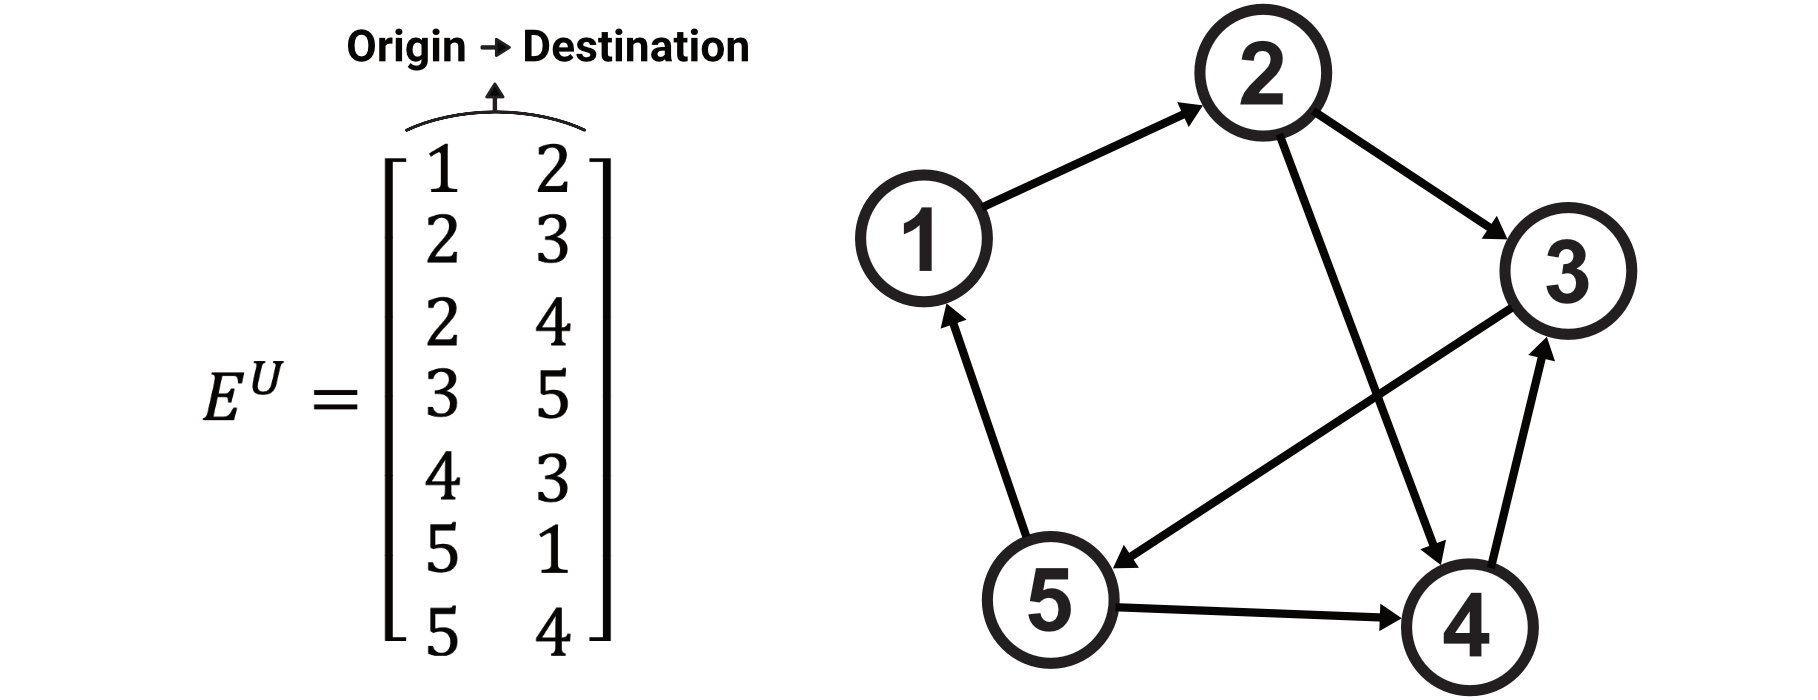
\includegraphics[width=1\linewidth,height=\textheight,keepaspectratio]{figures/fig-edge-list-unweighted.png}

}

\caption{\label{fig-edge-list-unweighted}Illustration of an edge list,
\(E^U\), and its corresponding network graph for an \textit{unweighted}
and \textit{directed} network of 5 nodes. In the edge list, each row
corresponds to an edge from an origin (first column) to a destination
(second column). In the network graph, circles indicate nodes and arrows
the edges between them.}

\end{figure}%

We take the roundwood trade network for each year of the data as a
weighted and directed network, \emph{i.e.}, we consider whether or not
two countries are connected by trade, the direction of the trade flows,
and the ``weight'' (or quantity/value) of the trade flows. In our case,
we consider the traded value to be the ``weight'' of the trade flow.
This is in contrast to using the net weight in metric tons, which is not
an appropriate unit of volume for roundwood as the mass of the roundwood
depends on its moisture content.\footnote{UN Comtrade data provides an
  alternative ``quantity'' variable (encoded \emph{qty}) to the net
  weight of the trade flows. However, this variable is poorly reported:
  (i) units may differ depending on the reporter and range from cubic
  metres to metres to kilograms, and so on; (ii) the ``quantity''
  variable is not recorded in 7.8\% of the dataset.} Due to data
discrepancies, the reported trade value from the exporter and importer
of the same trade flow may differ for at least two reasons: (1) import
reports are expressed as ``cost, insurance and freight'' (CIF), while
export reports are expressed as ``free on board'' (FOB), which excludes
CIF costs from trade value, leading to bilateral asymmetries; (2) one of
the trading partners may not report the trade
\citep{gaulier_baci_2010, rougieux_forest_2017, kallio_reliability_2018, chen_advancing_2022, mitikj_bridging_2024}.
To minimise the bias that such inconsistencies may cause, we consider
both the exporter's and importer's reports of trade: \(a_{o,d}\) and
\(a_{d,o}\), respectively. The edge list corresponding to the weighted,
directed trade network is now a matrix of size
\(N \times 4\).\footnote{In fact, edge lists are close to mirror flows
  that can be derived from bilateral trade data, such as that provided
  by the UN Comtrade database.} Each row represents a trade flow for a
given year \(t\), including the country of origin, the country of
destination, and the trade values reported by the exporter and importer,
as shown in Figure~\ref{fig-edge-list-weighted}.\footnote{See
  \citet{rayfield_connectivity_2011} and \citet{thompson_loss_2017} for
  examples of this approach in ecological networks.} We therefore define
28 edge lists to describe the roundwood trade network for each year of
trade.

\begin{figure}[t]

\centering{

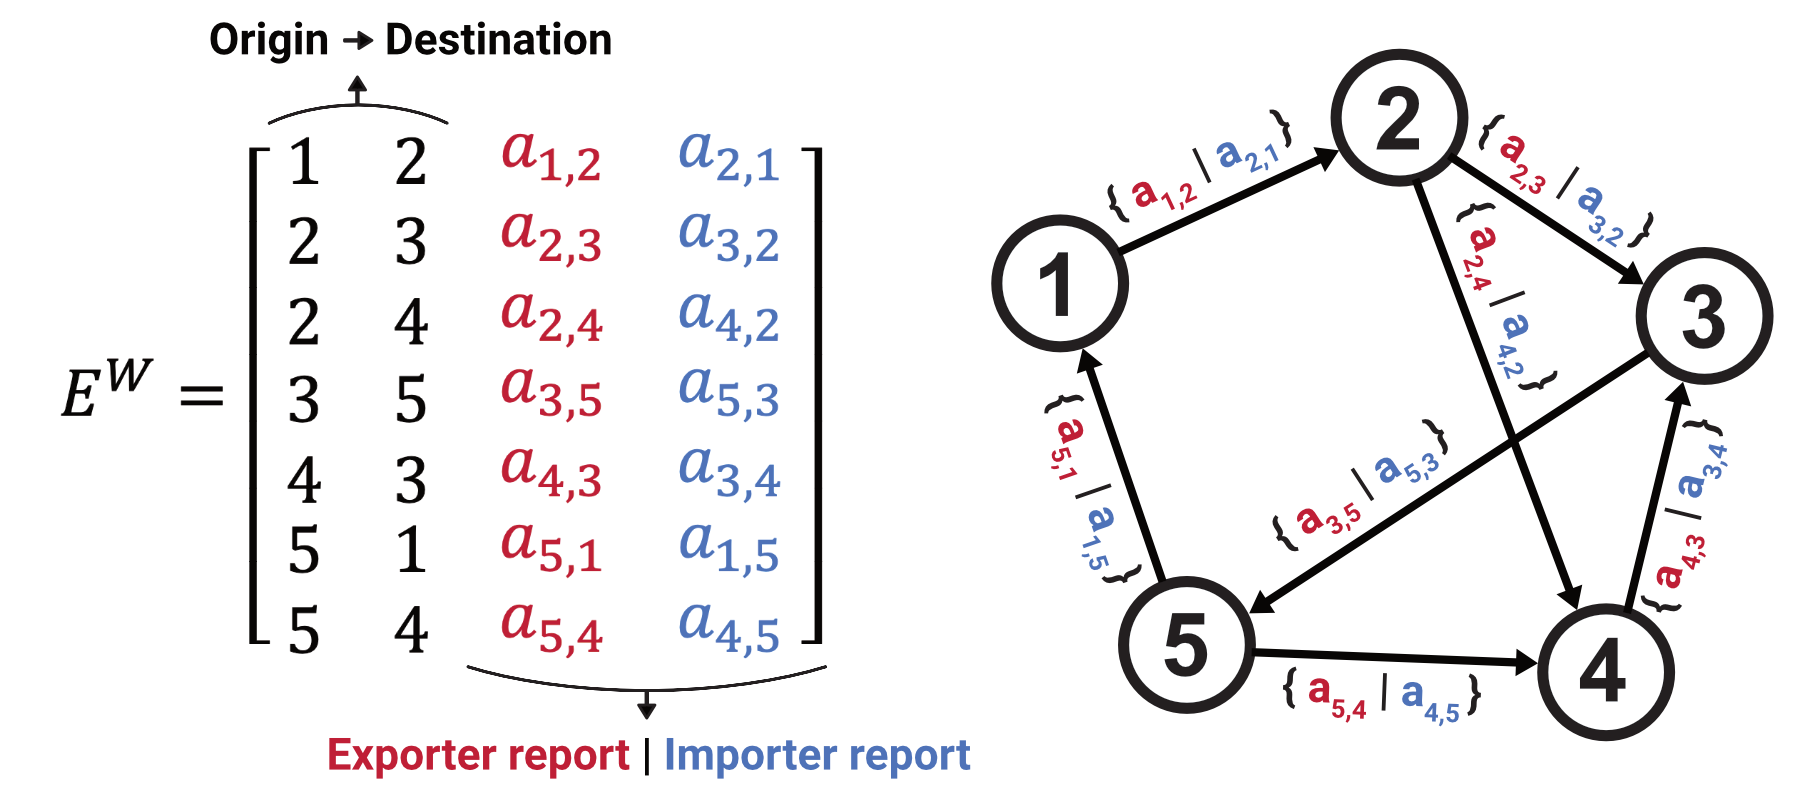
\includegraphics[width=1\linewidth,height=\textheight,keepaspectratio]{figures/fig-edge-list-weighted.png}

}

\caption{\label{fig-edge-list-weighted}Illustration of an edge list,
\(E^W\), and its corresponding network graph for a \textit{weighted} and
\textit{directed} trade network of 5 nodes. In the edge list, each row
corresponds to an edge from an origin (first column) to a destination
(second column) and include trade values reported by the country of
origin (third column, red) and the country of destination (fourth
column, blue). In the network graph, circles indicate nodes and arrows
the edges between them.}

\end{figure}%

\subsection{Trade network properties
assessment}\label{trade-network-properties-assessment}

Edge lists and any other network objects or raw visualisations are often
difficult to read and interpret. Alone, they do not enable a thorough
analysis of the structure of a trade network. In order to assess the
structural characteristics of trade networks, we computed a series of
network metrics for each year, differentiating between exports and
imports.\footnote{Considering directed networks enables analysis from
  either the origin (exporter) or destination (importer) country
  perspective, allowing exporter or importer trade behaviour to be
  inferred.} The Python package ``networkx'' 3.4.2
\citep{hagberg_exploring_2008} is used to facilitate the measurement
network metrics.

First, we assess the composition of the trade network. For each year, we
compute the total number of nodes in the network, \emph{i.e.}, the total
number of trading countries. These countries are then divided into three
more detailed groups: pure exporters (countries that only export
roundwood), pure importers (countries that only import roundwood) and
mixed countries (countries that both export and import roundwood). To
obtain more detailed information on the composition of the network, we
then cross-reference the export and import values of each trading
country accounting for at least 1\% of to the global export or import
value with the number of its export and import trading partners. This
provides country trade profiles for each year, allowing trade behaviours
and groups to be inferred and their evolution observed over time. This
set of metrics provides a general overview of the roundwood trade
network.

Secondly, to understand the finer details of the network structure, we
then computed a set of metrics that assess the connectivity of the trade
network, \emph{i.e.}, the mean, variance, skewness, and kurtosis of the
number of connections per node
\citep{albert_statistical_2002, newman_structure_2003}. Again, we assess
network connectivity differentiating exports and imports. The mean
number of connections per node, or node degree, is an average indicator
of the degree of connectedness of the network. A high mean number of
connections per node means that each country in the network has, on
average, a high number of trading partners. The variance of the number
of connections per node provides additional information about the
dispersion of the number of connections. If the variance is close to
zero, then the nodes in the network have more or less the same degree. A
high variance indicates that the degree of connectivity of countries
largely deviates from the mean. Skewness provides information about the
proportion of low to highly connected nodes in the network. If the
skewness is negative, the network consists of a higher proportion of
highly connected nodes. Conversely, if the skewness is positive, then
the network has a higher proportion of lowly connected nodes. Zero
skewness implies an equal ratio of low to high connected nodes. Kurtosis
provides information on how the degree distribution compares with a
normal distribution in terms of its ``tailedness'' or ``flatness''. A
positive kurtosis\footnote{We consider Fisher's definition of kurtosis.
  A Pearson's definition would have necessitated the comparison of
  kurtosis values with 3 instead of 0.} indicates that tailed outliers
are more prevalent than in a normal distribution, meaning countries that
diverge from the mean are rare. Conversely, negative kurtosis
corresponds to a situation in which outliers are common, \emph{i.e.},
where most countries diverge from the mean.

Lastly, we assess market concentration by combining our network approach
with a traditional Herfindahl-Hirschman market concentration index
(HHI). The HHI is defined as follows:

\begin{equation}\phantomsection\label{eq-HHI}{
HHI = \sum^{N}_{i = 1} (MS_{i})^{2}
}\end{equation}

where \(N\) is the number of countries involved in trade and \(MS_{i}\)
the market share of the country \(i\), that is, the ratio of the value
traded by country \(i\) to the global value traded. We computed two
\(HHI\), one for exports and one for imports. The \(HHI\) values can
range from \(1/N\) to 1. According to the \(HHI\) value, the US Federal
Trade Commission differentiates three types of markets
\citep{us_department_of_justice_and_the_federal_trade_commission_horizontal_2010}:

\begin{itemize}
\tightlist
\item
  An \(HHI\) between 0.01 and 0.15 corresponds to an unconcentrated
  market, \emph{i.e.}, a market with no anti-competitive effects
  presumed;
\item
  An \(HHI\) between 0.15 and 0.25 indicates a moderately concentrated
  market, \emph{i.e.}, a market with potential or significant
  anti-competitive effects;
\item
  An \(HHI\) greater than 0.25 indicates a highly concentrated market,
  \emph{i.e.}, a market with presumption of anti-competitive effects.
\end{itemize}

To obtain a more detailed understanding of market concentration, we
calculated each country's annual contribution to the global trade value,
\emph{i.e.}, the reduction in total trade value if a given country were
removed from the network. This is equivalent to estimating the share of
total trade value that ``flows'' through a given country in a particular
year. Consequently, the sum of all countries' contributions does not add
up to 100\%, due to the bilateral nature of trade flows. This approach
allows us to identify dominant countries in the roundwood trade. In
cases of high market concentration, the removal of a dominant country is
expected to result in a substantial loss in trade value.

Combining multiple complementary metrics offers a more comprehensive
understanding of the network's structure than any single metric alone
can provide \citep{shanafelt_-it-yourself_2017, salau_taking_2022}. For
example, networks may have the same average number of connections but
exhibit vastly different variances, resulting in markedly different
topologies. Moreover, we consider our selected set of metrics sufficient
for analyzing trade network structure, as many network metrics tend to
be correlated \citep{baggio_landscape_2011}. The metrics used and their
interpretations are summarized in Table~\ref{tbl-network-metrics}.

\begin{longtable}[]{@{}
  >{\raggedright\arraybackslash}p{(\linewidth - 2\tabcolsep) * \real{0.4286}}
  >{\raggedright\arraybackslash}p{(\linewidth - 2\tabcolsep) * \real{0.5714}}@{}}
\caption{List of the metrics used to describe the trade network and
their interpretation.}\label{tbl-network-metrics}\tabularnewline
\toprule\noalign{}
\begin{minipage}[b]{\linewidth}\raggedright
Network metrics
\end{minipage} & \begin{minipage}[b]{\linewidth}\raggedright
Interpretation
\end{minipage} \\
\midrule\noalign{}
\endfirsthead
\toprule\noalign{}
\begin{minipage}[b]{\linewidth}\raggedright
Network metrics
\end{minipage} & \begin{minipage}[b]{\linewidth}\raggedright
Interpretation
\end{minipage} \\
\midrule\noalign{}
\endhead
\bottomrule\noalign{}
\endlastfoot
\textbf{Trade network composition} & \\
Number of nodes & Number of countries involved in trade. \\
Number of pure exporter & Number of countries that only export
roundwood. \\
Number of pure importer & Number of countries that only import
roundwood. \\
Number of mixed countries & Number of countries that both export and
import roundwood. \\
Country profiles & Trade behaviour of countries in relation to exports
and imports. \\
\textbf{Trade network connectivity} & \\
Mean number of connections per node & Average number of trading partners
per country; indicator of the overall connected-ness of the network. \\
Variance in the number of connections per node & Variation in the number
of trading partners relative to the mean. \\
Skewness in the number of connections per node & Proportion of low to
highly connected countries in the network. \\
Kurtosis in the number of connections per node & Scarcity or abundance
of countries that diverge from the mean connectivity. \\
\textbf{Market concentration} & \\
Herfindahl-Hirschman index & Market concentration in the trade of
roundwood. \\
Country contributions to trade value & Share of total trade value that
`flows' through a given country. \\
\end{longtable}

\subsection{Computational workflow and
reproducibility}\label{computational-workflow-and-reproducibility}

A sustainable data analysis workflow was undertaken using Snakemake
9.6.0 \citep{molder_sustainable_2025}. Snakemake is a workflow
management system that ensures the reproducibility, adaptability, and
transparency of the data analysis. This workflow is available on a
GitHub repository,\footnote{GitHub repository address:
  \url{https://github.com/vlmathieu/trade_network_analysis}} which
provides access to the analysis and version control
\citep{braga_not_2023}.

\section{Results}\label{results}

\subsection{Composition of the trade network over
time}\label{composition-of-the-trade-network-over-time}

Over the study period, the number of countries involved in the roundwood
trade fluctuated slightly, ranging from 189 in 1997 to 214 in 2008
(Figure~\ref{fig-network-composition}). On average, 206 countries were
involved in roundwood trade from 1996 to 2023. After a moderate increase
in the number of countries involved in trade between 1996 and 2008 (an
increase of 11.5\%, from 192 to 214 countries), the number of countries
stabilised until 2015. From 2015 to 2022, the number of trading
countries decreased slightly from 213 to 198 (an 7\% decrease) before
increasing to 209 in 2023 (an increase of 5.3\%). Aside from these
trends, we found short-term slight decreases in the number of trading
countries after 2008, 2015, 2019, and 2021, which, as we will discuss
later, can likely be attributed to major global events.

In addition, we can observe several trends in the share of pure
exporters, pure importers, and countries that both export and import
roundwood. The number of pure exporters has decreased markedly since
1996, falling from 17 to 11 (a decline of around 35.3\%). In 2023, pure
exporters represented only 5.3\% of trading countries compared to an
average of 6.3\% over the studied period. In contrast, the number of
pure importers decreased from 52 to 39 between 1996 and 2007 (a decline
of 25\%), before rising again to 60 between 2007 and 2015 (an increase
of 53.8\%). Since 2015, the number of pure importers has stabilised
around 55 countries on average. In 2023, pure importers represented a
larger share (28.7\%, 60 countries) of trading countries than pure
exporters (23.5\% on average over the study period). Throughout the
years, there were consistently more pure importers than pure exporters
engaged in the international trade of roundwood, with an average
difference of 36 countries. The number of countries that both export and
import roundwood (``mixed countries'') constituted the vast majority of
trading countries (70.2\% on average over the studied period, 66\% in
2023). The number of mixed countries has increased moderately since
1996, rising from 123 to 138 (an increase of around 12.2\%). As for the
total number of trading countries, we noticed short terms drops in the
number of pure exporters, pure importers, and mixed countries over the
studied period. Some drops are common to pure importers and mixed
countries (\emph{e.g.}, following 2008 and 2019), while others are
group-specific (\emph{e.g.}, following 1997 for pure exporters and 2001
for pure importers).

\begin{figure}[t]

\centering{

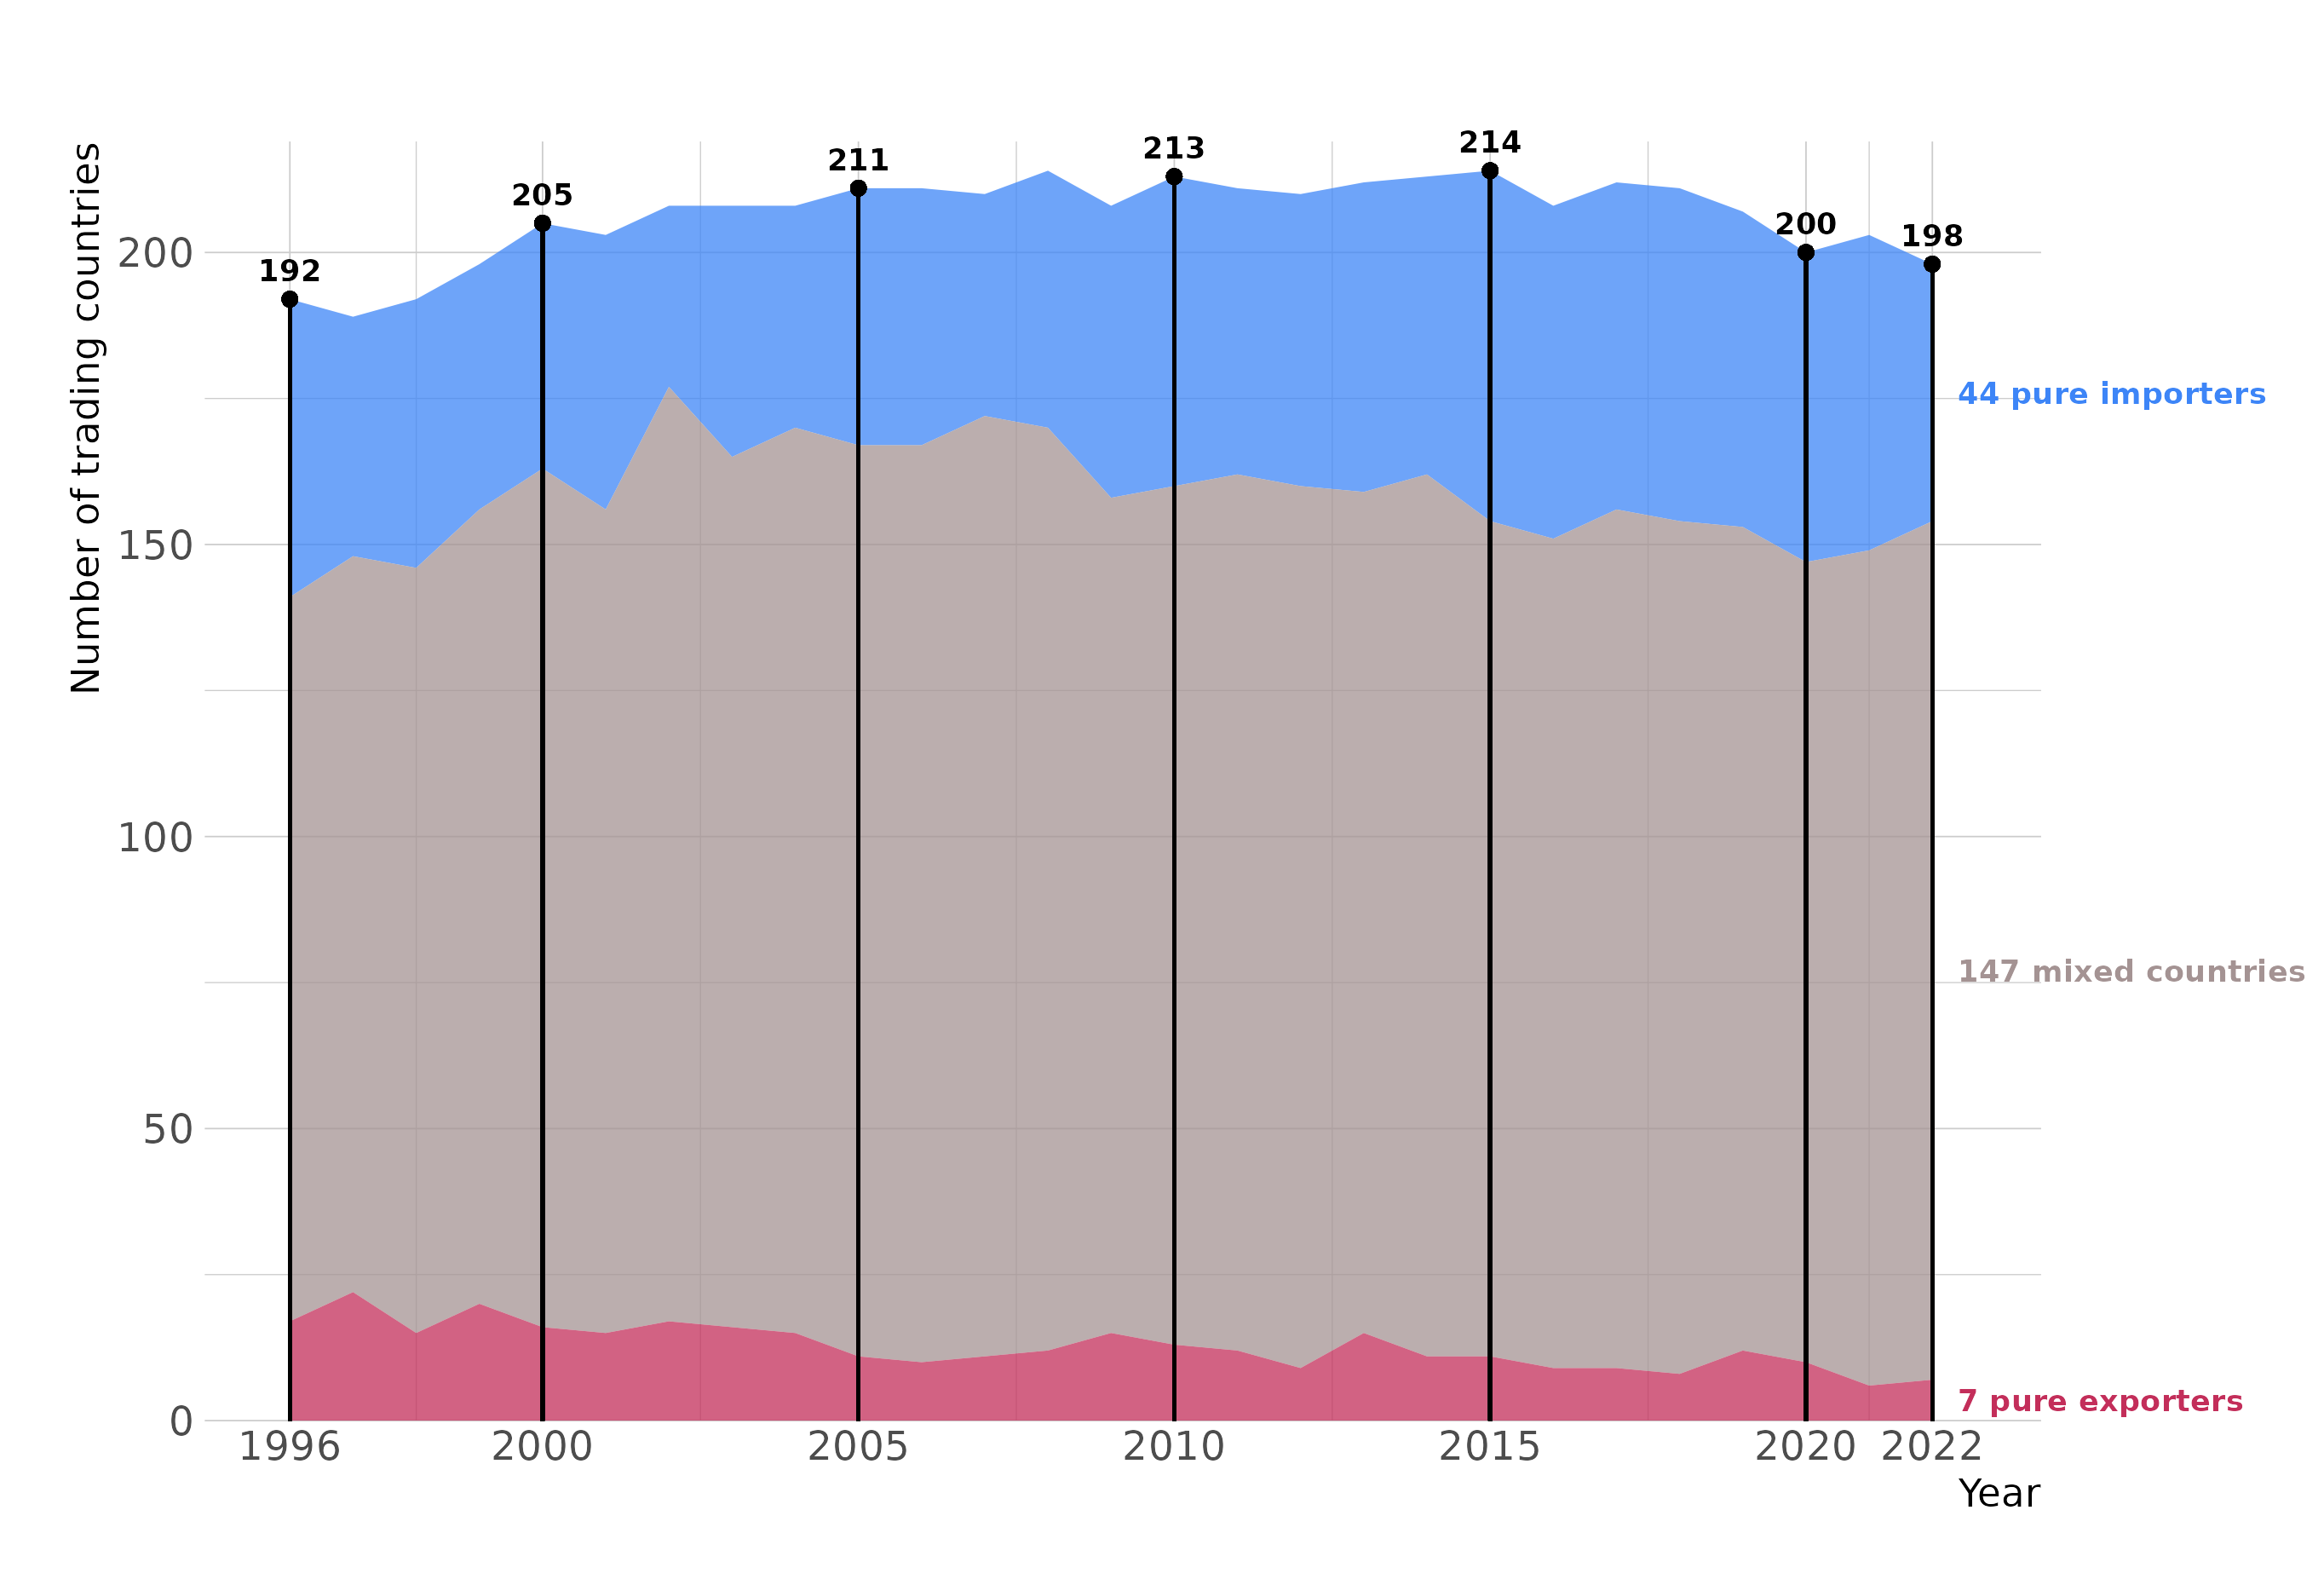
\includegraphics[width=1\linewidth,height=\textheight,keepaspectratio]{figures/fig-network-composition.png}

}

\caption{\label{fig-network-composition}Number of trading countries in
total and per group: pure exporters (red), pure importers (blue), mixed
countries (grey); for each year of trade.}

\end{figure}%

While 200 countries were involved in the global roundwood trade in 2020,
only 31 countries (15.5\% of the total) contributed to at least 1\% of
the export or import value (Figure~\ref{fig-countries-profiles}). This
suggests a certain degree of market concentration in the trade of
roundwood. These 31 countries showed different behaviours, and we
identified roughly three groups. First, Asian countries, namely China,
India, Japan, the Republic of Korea and Vietnam, form a group of
importers. Importers have a higher trade value for imports than for
exports and have diversified their import connections more than their
export connections. Second, several countries belong to the group of
exporters. Their export value is higher than their import value, they
have a higher number of export partners compared to their import
partners, but their number of export trading partners varies. While
Papua New Guinea only export to a limited number of 13 countries, net
exporters such as Australia, New Zealand, Congo, Cameroon, Brazil and
the Russian Federation, have moderately diversified their number of
export trading partners (between 20 and 45). New Zealand, the USA, and
the Russian Federation stand out as the world's three largest suppliers
of roundwood. In particular, the USA shows a unique export pattern with
a high diversification of its export trading partners (95 export
connections). Finally, we can draw a third group of countries that tend
to export as much as they import in trade value, with a balanced number
of exporting and importing partners. This group is mainly made up of
European countries but also includes countries such as Canada and
Malaysia.

The trade situation has changed significantly between 2000 and 2020
(Figure~\ref{fig-countries-profiles}). In 20 years, China has overtaken
Japan as the main importer of roundwood. Japan's import value decreased
dramatically from more than \$2.33 billion in 2000 to about \$562
million in 2020, a decrease of 76\%. On the other hand, China's import
value increased considerably from more than \$1.654 billion in 2000 to
more than \$8.376 billion in 2020, an increase of about 406\%.
Surprisingly, the number of China's export trading partners increased
sharply by about 129\% between 2000 and 2020 (31 new export trading
partners), while the value of Chinese export trade decreased by more
than \$1.2 million on the same period (a decline of about 16\%), which
seems unlikely. In terms of trade value, New Zealand has emerged as the
world's top exporter of roundwood, while maintaining a relatively stable
number of trading partners. Although the USA and the Russian Federation
remained major exporters of roundwood, they appeared to be less
integrated into global roundwood trade. Between 2000 and 2020, the USA
has lost a large share of its trading partners to import (a fall of
42\%), while slightly reducing its export diversification (a fall of
only 8\%). Similarly, the Russian Federation lost 14 export trading
partners (25\%) and 5 import trading partners (42\%) in the same period.

\begin{figure}[p]

\centering{

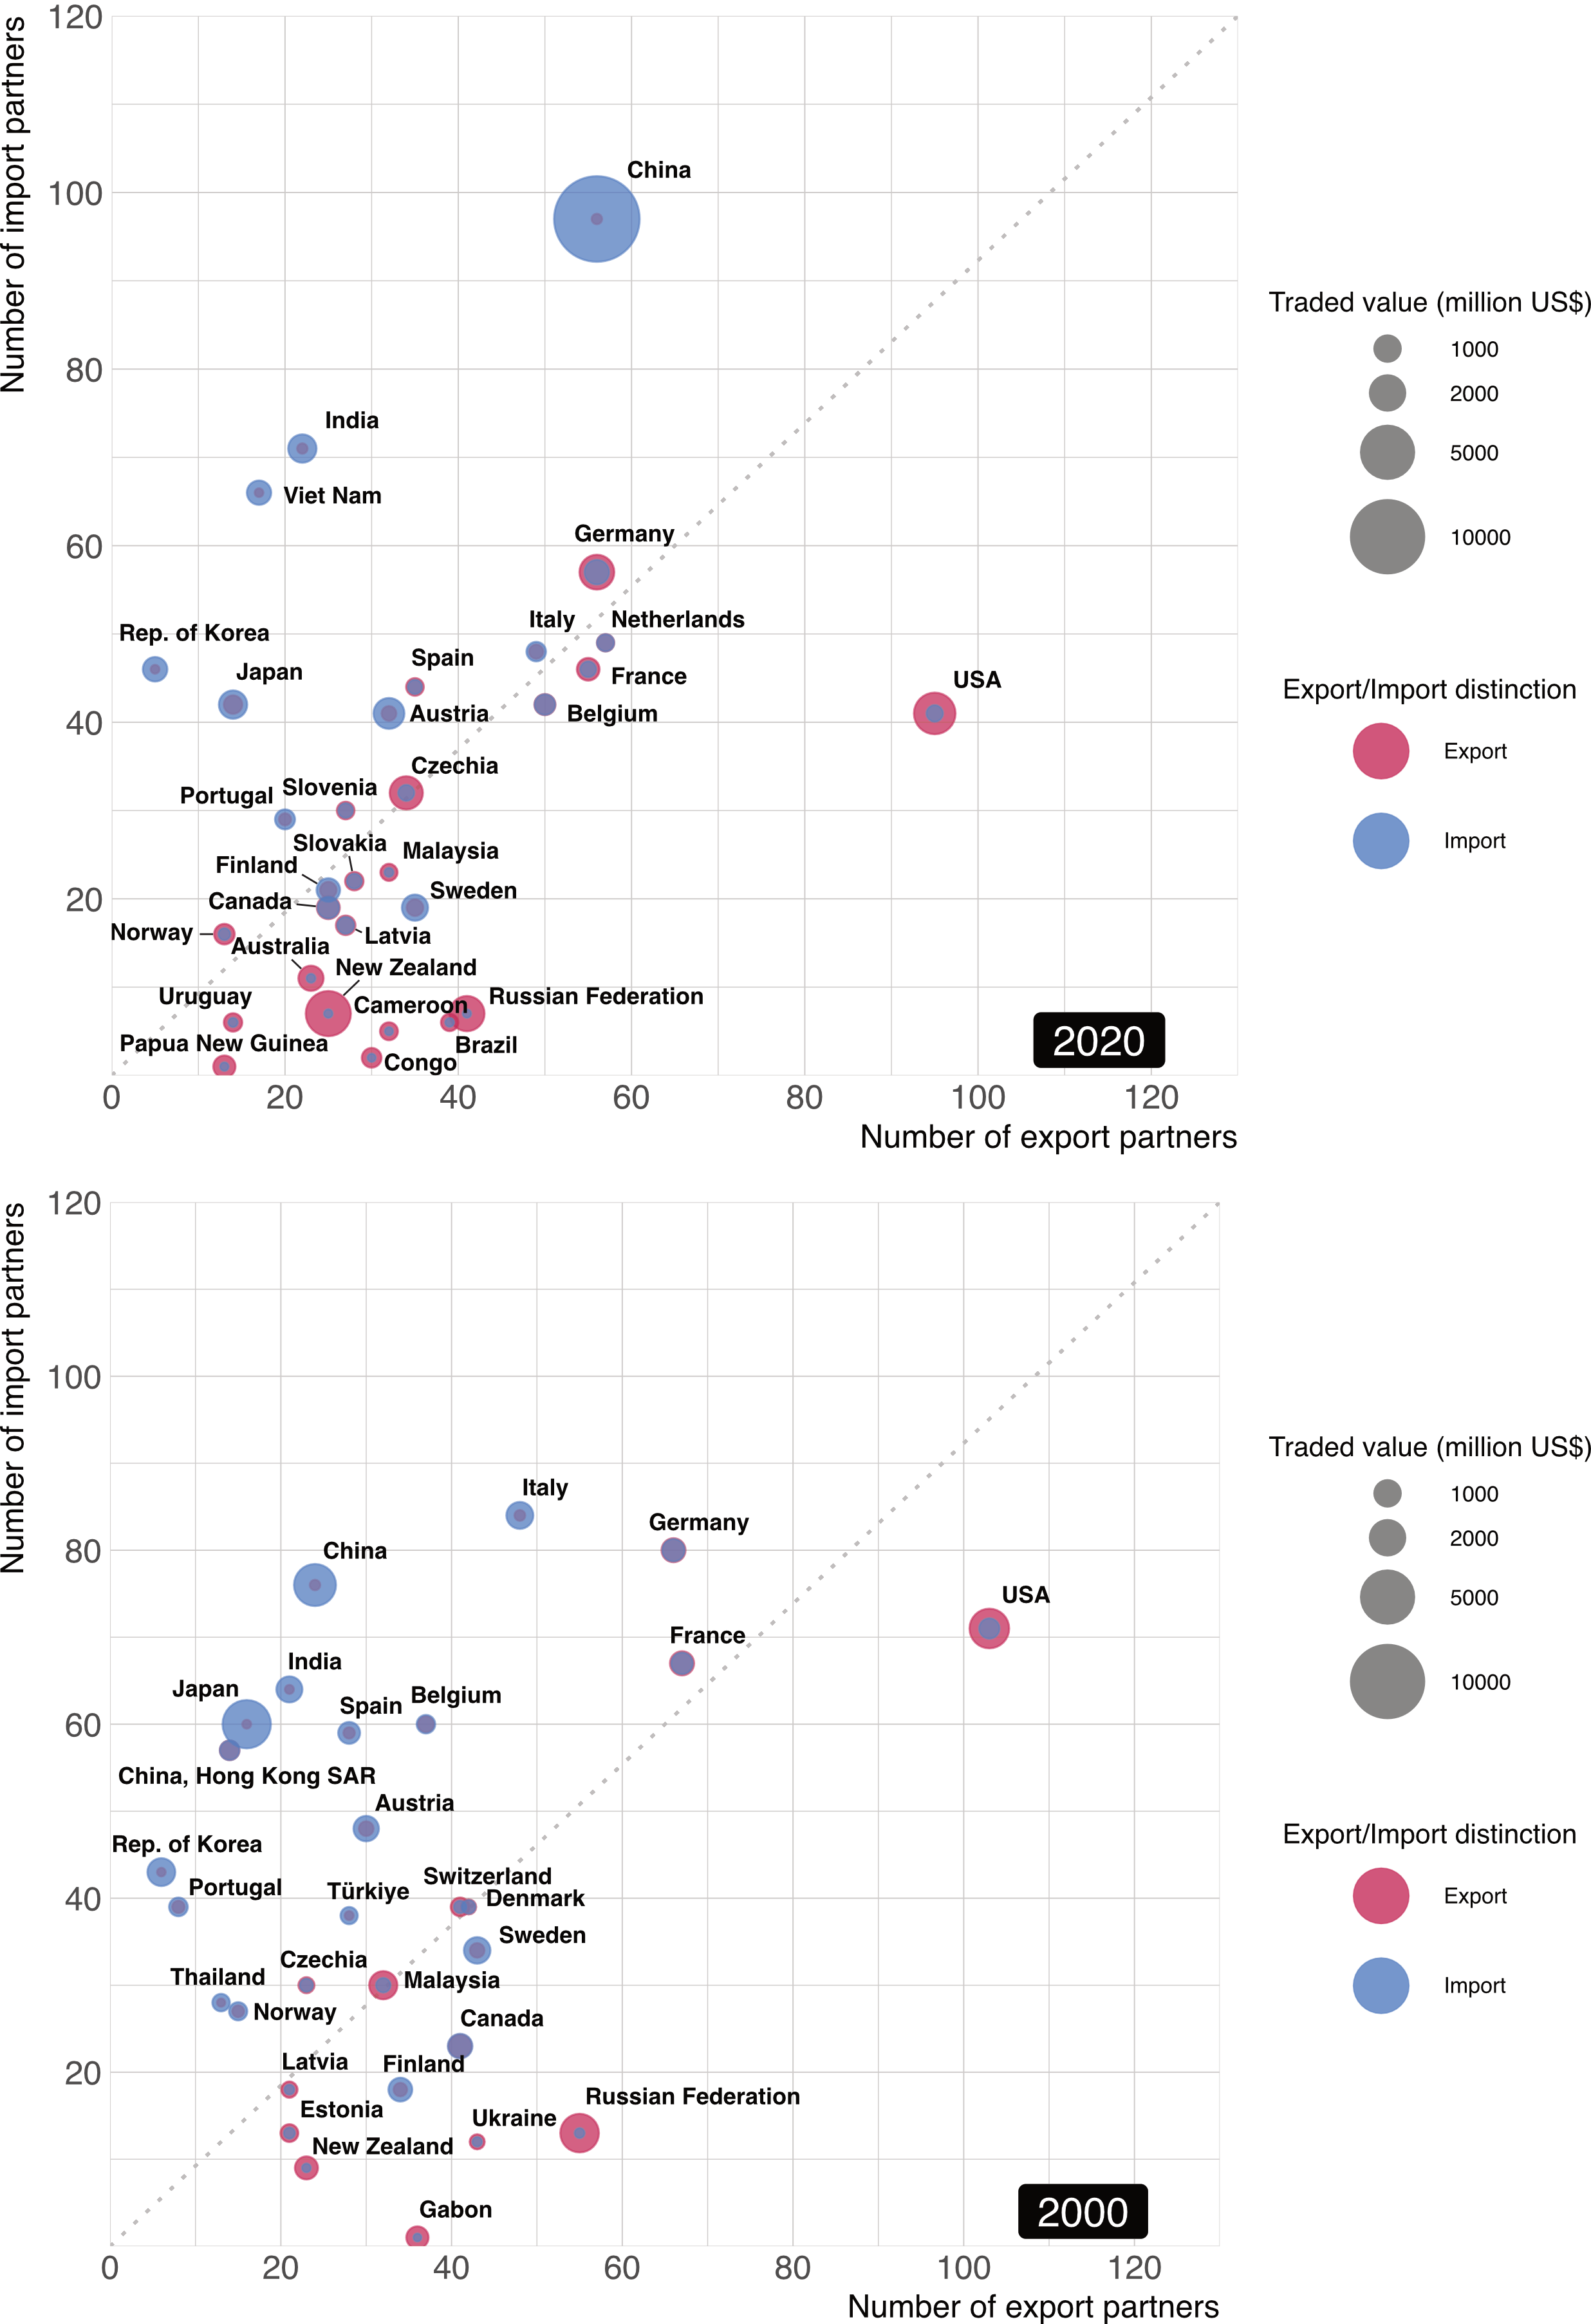
\includegraphics[width=\linewidth,height=0.9\textheight,keepaspectratio]{figures/fig-countries-profiles.png}

}

\caption{\label{fig-countries-profiles}Bubble graph showing the profiles
of trading countries in 2020 (top) and in 2000 (bottom). Countries are
displayed according to the number of partners with whom the trade
exports and imports. The size of the bubbles increases with the value of
trade. Blue bubbles refer to imports and red bubbles refer to exports.
Only countries accounting for at least 1\% of the value of exports or
imports in 1996 or 2022 are shown.}

\end{figure}%

\subsection{Connectivity of the trade network over
time}\label{connectivity-of-the-trade-network-over-time}

\begin{figure}[t]

\centering{

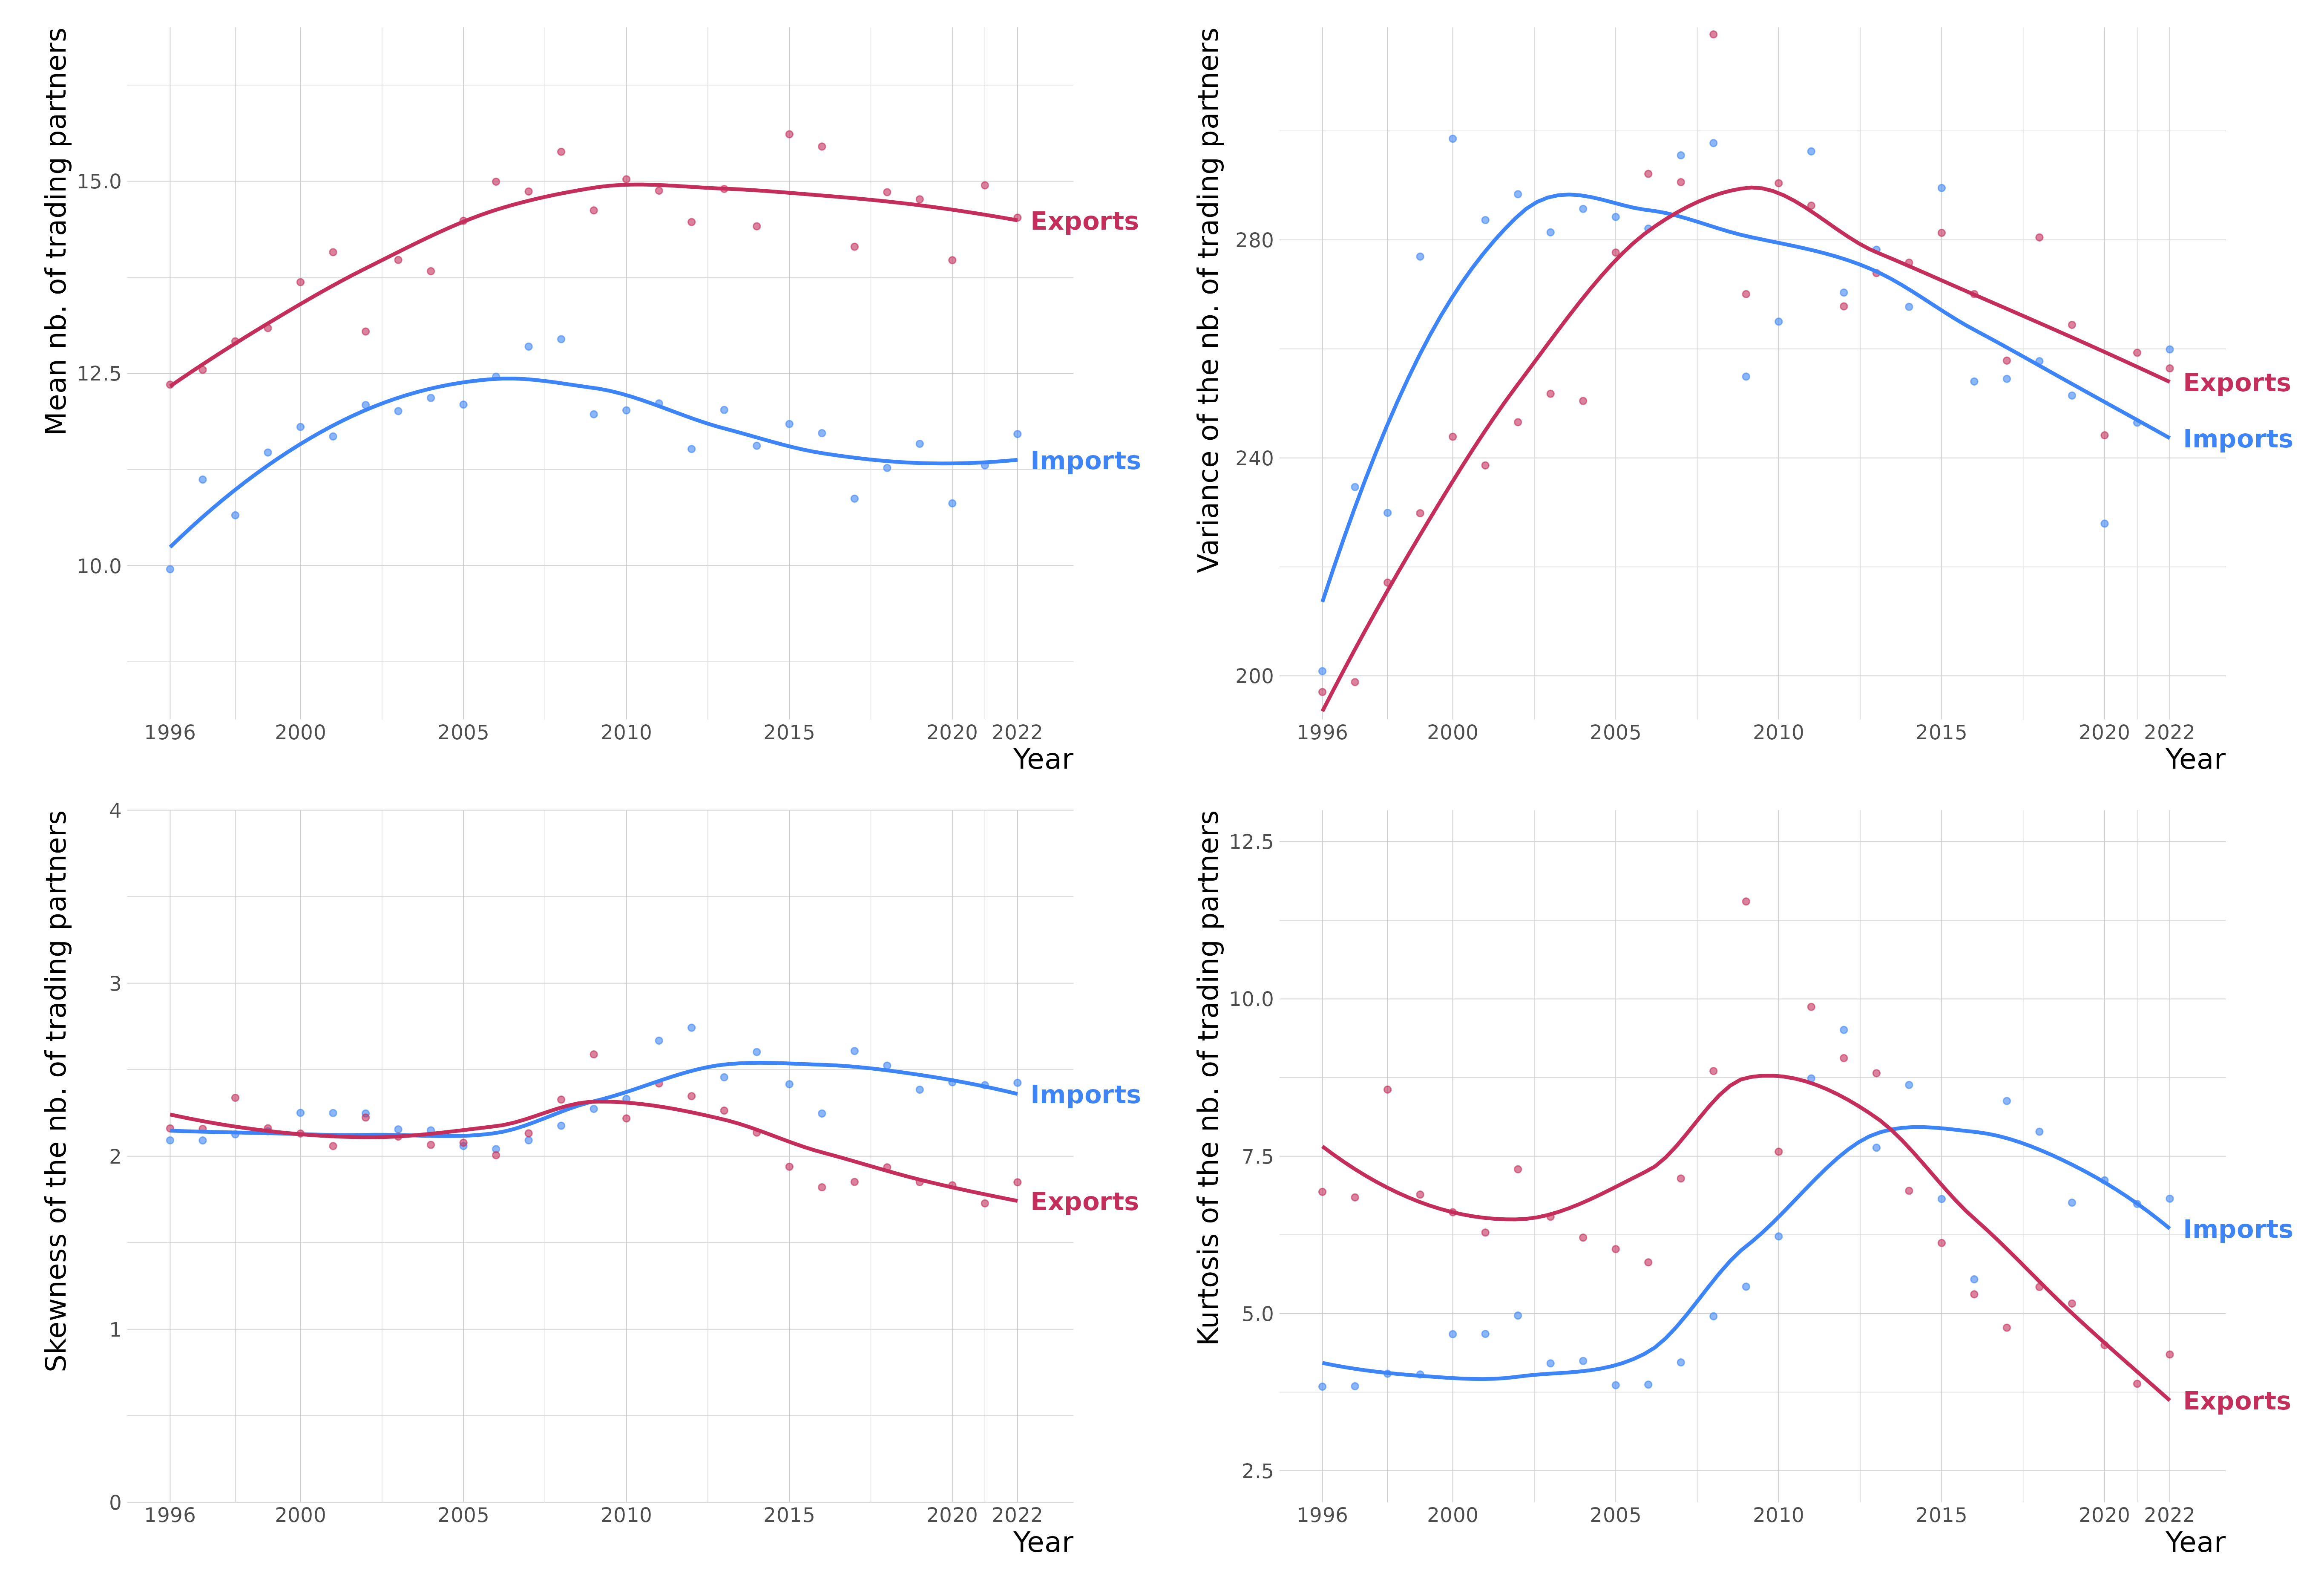
\includegraphics[width=1\linewidth,height=\textheight,keepaspectratio]{figures/fig-network-connectivity.png}

}

\caption{\label{fig-network-connectivity}Mean number (top left),
variance (top right), skewness (bottom left), and kurtosis (bottom
right) of the connections per node. Metrics concerning exports are
plotted in red, metrics concerning imports are plotted in blue. Smooth
curve is based on a Loess function to highlight trends in the metrics.}

\end{figure}%

Results for mean, variance, skewness, and kurtosis of the connections
per country are presented in Figure~\ref{fig-network-connectivity}.
Three general observations can be made regarding the average number of
connections per country over time. Firstly, both exporters and importers
of roundwood observed an increase in their mean connectivity during the
first half of the study period (from 1996 to 2008). During this period,
mean connectivity of exporters increased by 23\% for exporters (from
12.4 to 15.3 connections per exporter), while that of importers
increased by 30\% (from 9.9 to 12.9 connections per importer). The
average number of connections per country then slightly decreased by 8\%
for exporters (from 15.3 to 14.1). Mean connectivity of importers
decreased further by 18\% (from 12.9 to 10.6 connections per importer)
from 2008 to 2016 and has since stabilised. Secondly, exporters were, on
average, 23\% more connected than importers throughout the study period
(14.2 connections per exporter versus 11.6 connections per importer).
The gap widened between the first and second halves of the study period
(17\% between 1996 and 2008, 27\% between 2008 and 2023). Thirdly, aside
from general trends, short-term increases and decreases in mean
connectivity were observed from year to year, with some shared by both
by exporters and importers. For example, mean connectivity of both
exporters and importers dropped in the years following 2008, 2016, and
2019.

The variance in the number of connections per node provides additional
information on how the connectivity of each country diverges from the
overall average. Overall, we observe high variance in connectivity per
country for exporters and importers. Exporters and importers comprise
countries with a wide range of trading partners, some of which have a
significantly lower number of connections than average (poorly connected
countries), while others have a significantly higher number of
connections than average (highly connected countries). Variance in the
connectivity per country increased for importers from 1996 to 2003 and
for exporters until 2008, before decreasing until 2023. Between 1996 and
2005, variance in connectivity per country was, on average, higher for
importers than for exporters. This suggests that, during this time
period, importers showed greater spread in connectivity compared to the
mean. After 2005, exporters and importers displayed similar variances in
connectivity. Similar short-term increases and decreases to those
observed in mean connectivity per node were seen in the variance from
year to year.

Skewness provides information about the distribution of highly and
poorly connected nodes within a network. Skewness in connections per
country is always positive for both exporters and importers, indicating
a greater proportion of countries with low to high connectivity. It
remained stable on average for both exporters and importers between 1996
and 2005, followed by an increase until 2010 for exporters and until
2012 for importers. Until 2010, the degree of skewness in connectivity
was similar for exporters and importers. Since 2010, the skewness in
connectivity has become, on average, higher for importers than for
exporters, has slightly increased for importers, and has decreased
moderately for exporters. That is, there was a greater proportion of
poorly connected countries among importers than among exporters, which
supports and complements our findings regarding the mean number of
connections.

Kurtosis indicates whether countries diverge from the mean connectivity
in a scarce or abundant manner. During the study period, kurtosis of
connections per country remained positive for both exporters and
importers. This suggests that countries whose connectivity diverges from
the mean connectivity are rarer than those whose connectivity is close
to the mean. From 1996 to 2014, skewness of connectivity was higher for
exporters than for importers, meaning that exporters diverging from the
mean connectivity were, on average, rarer than importers. The reverse
was true after 2014. Until 2023, kurtosis of connectivity decreased,
while remaining positive. This fall is steeper for exporters than for
importers. As with our other network metrics, we observed several
short-term fluctuations in skewness and kurtosis over time from year to
year, though these were less pronounced.

\subsection{Market concentration in roundwood trade over
time}\label{market-concentration-in-roundwood-trade-over-time}

\begin{figure}[t]

\centering{

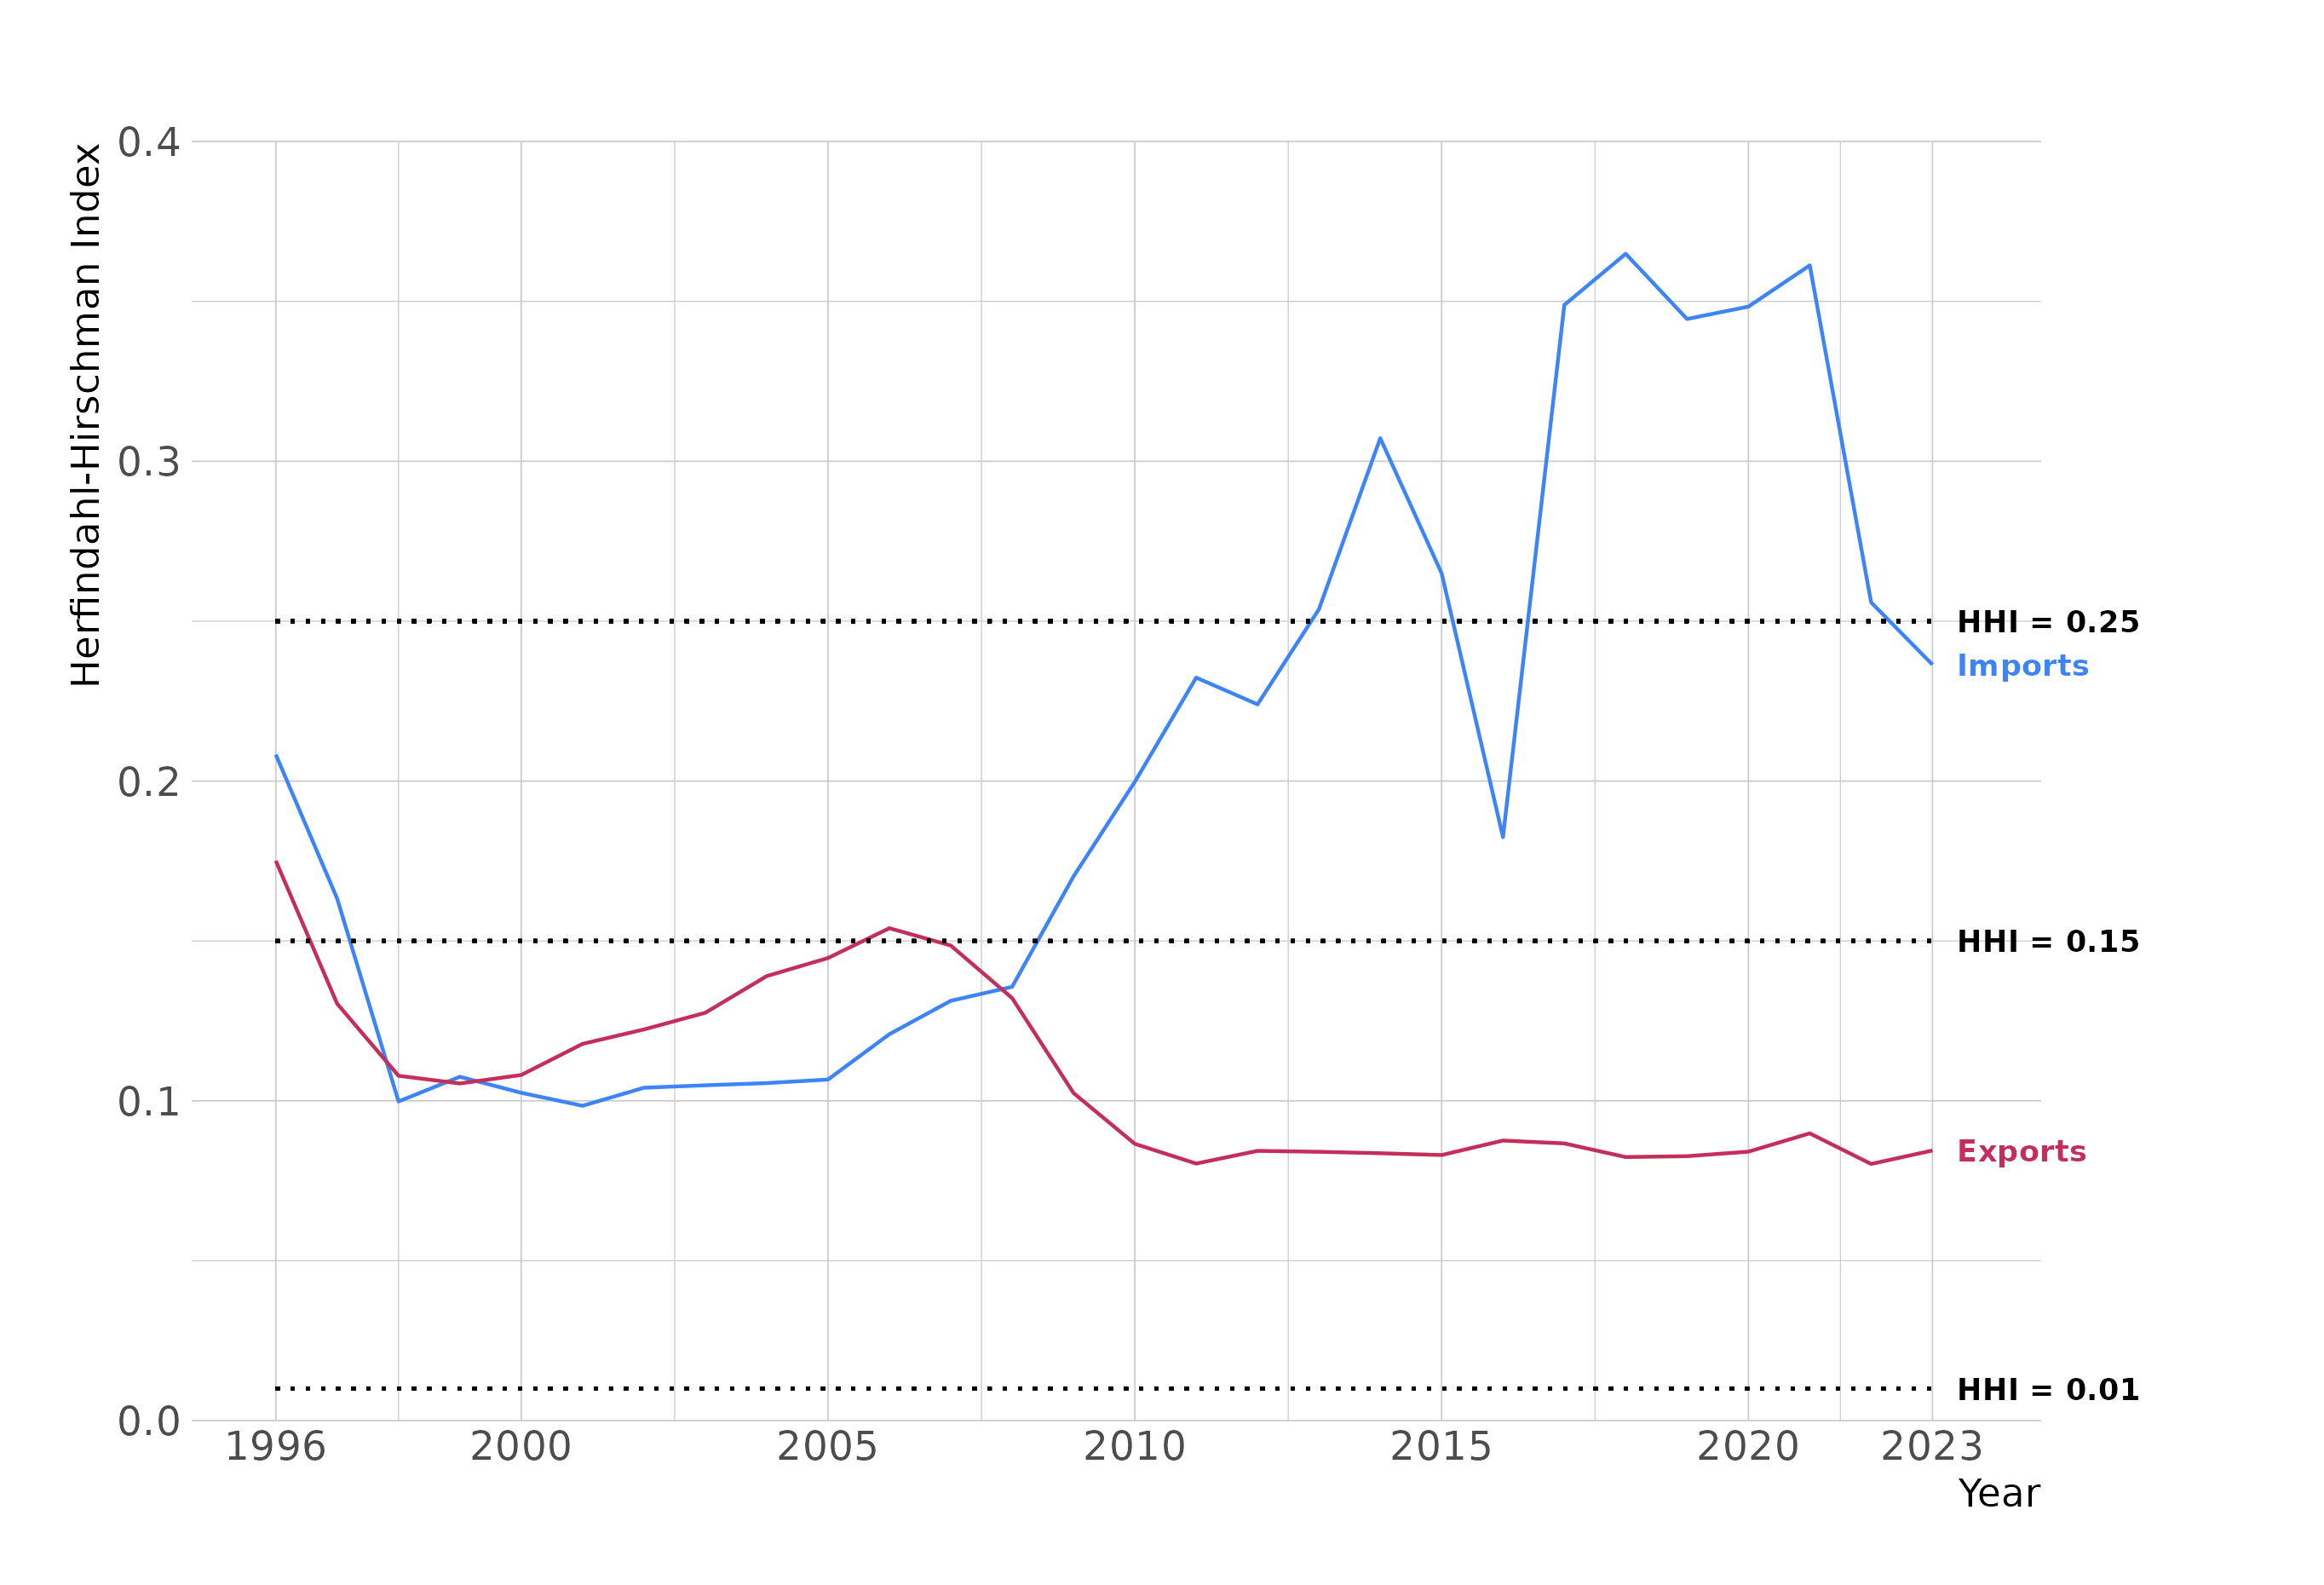
\includegraphics[width=1\linewidth,height=\textheight,keepaspectratio]{figures/fig-market-concentration.png}

}

\caption{\label{fig-market-concentration}Herfindahl-Hirschman index
values over time. Index related to exports are displayed in red, those
related to imports in blue.}

\end{figure}%

Between 1996 and 1998, the Herfindahl-Hirschman Index (HHI) initially
fell for both exports (a decline of 38\%, from 0.18 to 0.11) and imports
(a decline of 52\%, from 0.21 to 0.1) indicating a rapid shift from
moderate to low market concentration in roundwood trade
(Figure~\ref{fig-market-concentration}). This decline was followed by an
increase in the HHI for exporters until 2006, reaching a HHI of 0.15,
before falling again until 2011 and reaching a HHI of 0.08. Market of
roundwood exports then remained stable and lowly concentrated until
2023, with an average HHI of 0.08 since 2011. In contrast, market
concentration of roundwood imports increased sharply, becoming
moderately concentrated after 2009 (HHI of 0.17) and highly concentrated
after 2013 (HHI of 0.25). After a steep decline from a HHI of 0.26 to
0.18 between 2015 and 2016, market concentration level recovered the
following year to reach a HHI of 0.35. From 2017 to 2021, imports
remained highly concentrated, with an average HHI of 0.35, before
falling to 0.24 in 2023. On average, over the last decade, imports have
remained highly concentrated, whereas exports have remained lowly
concentrated for 27 years.

\begin{figure}[p]

\centering{

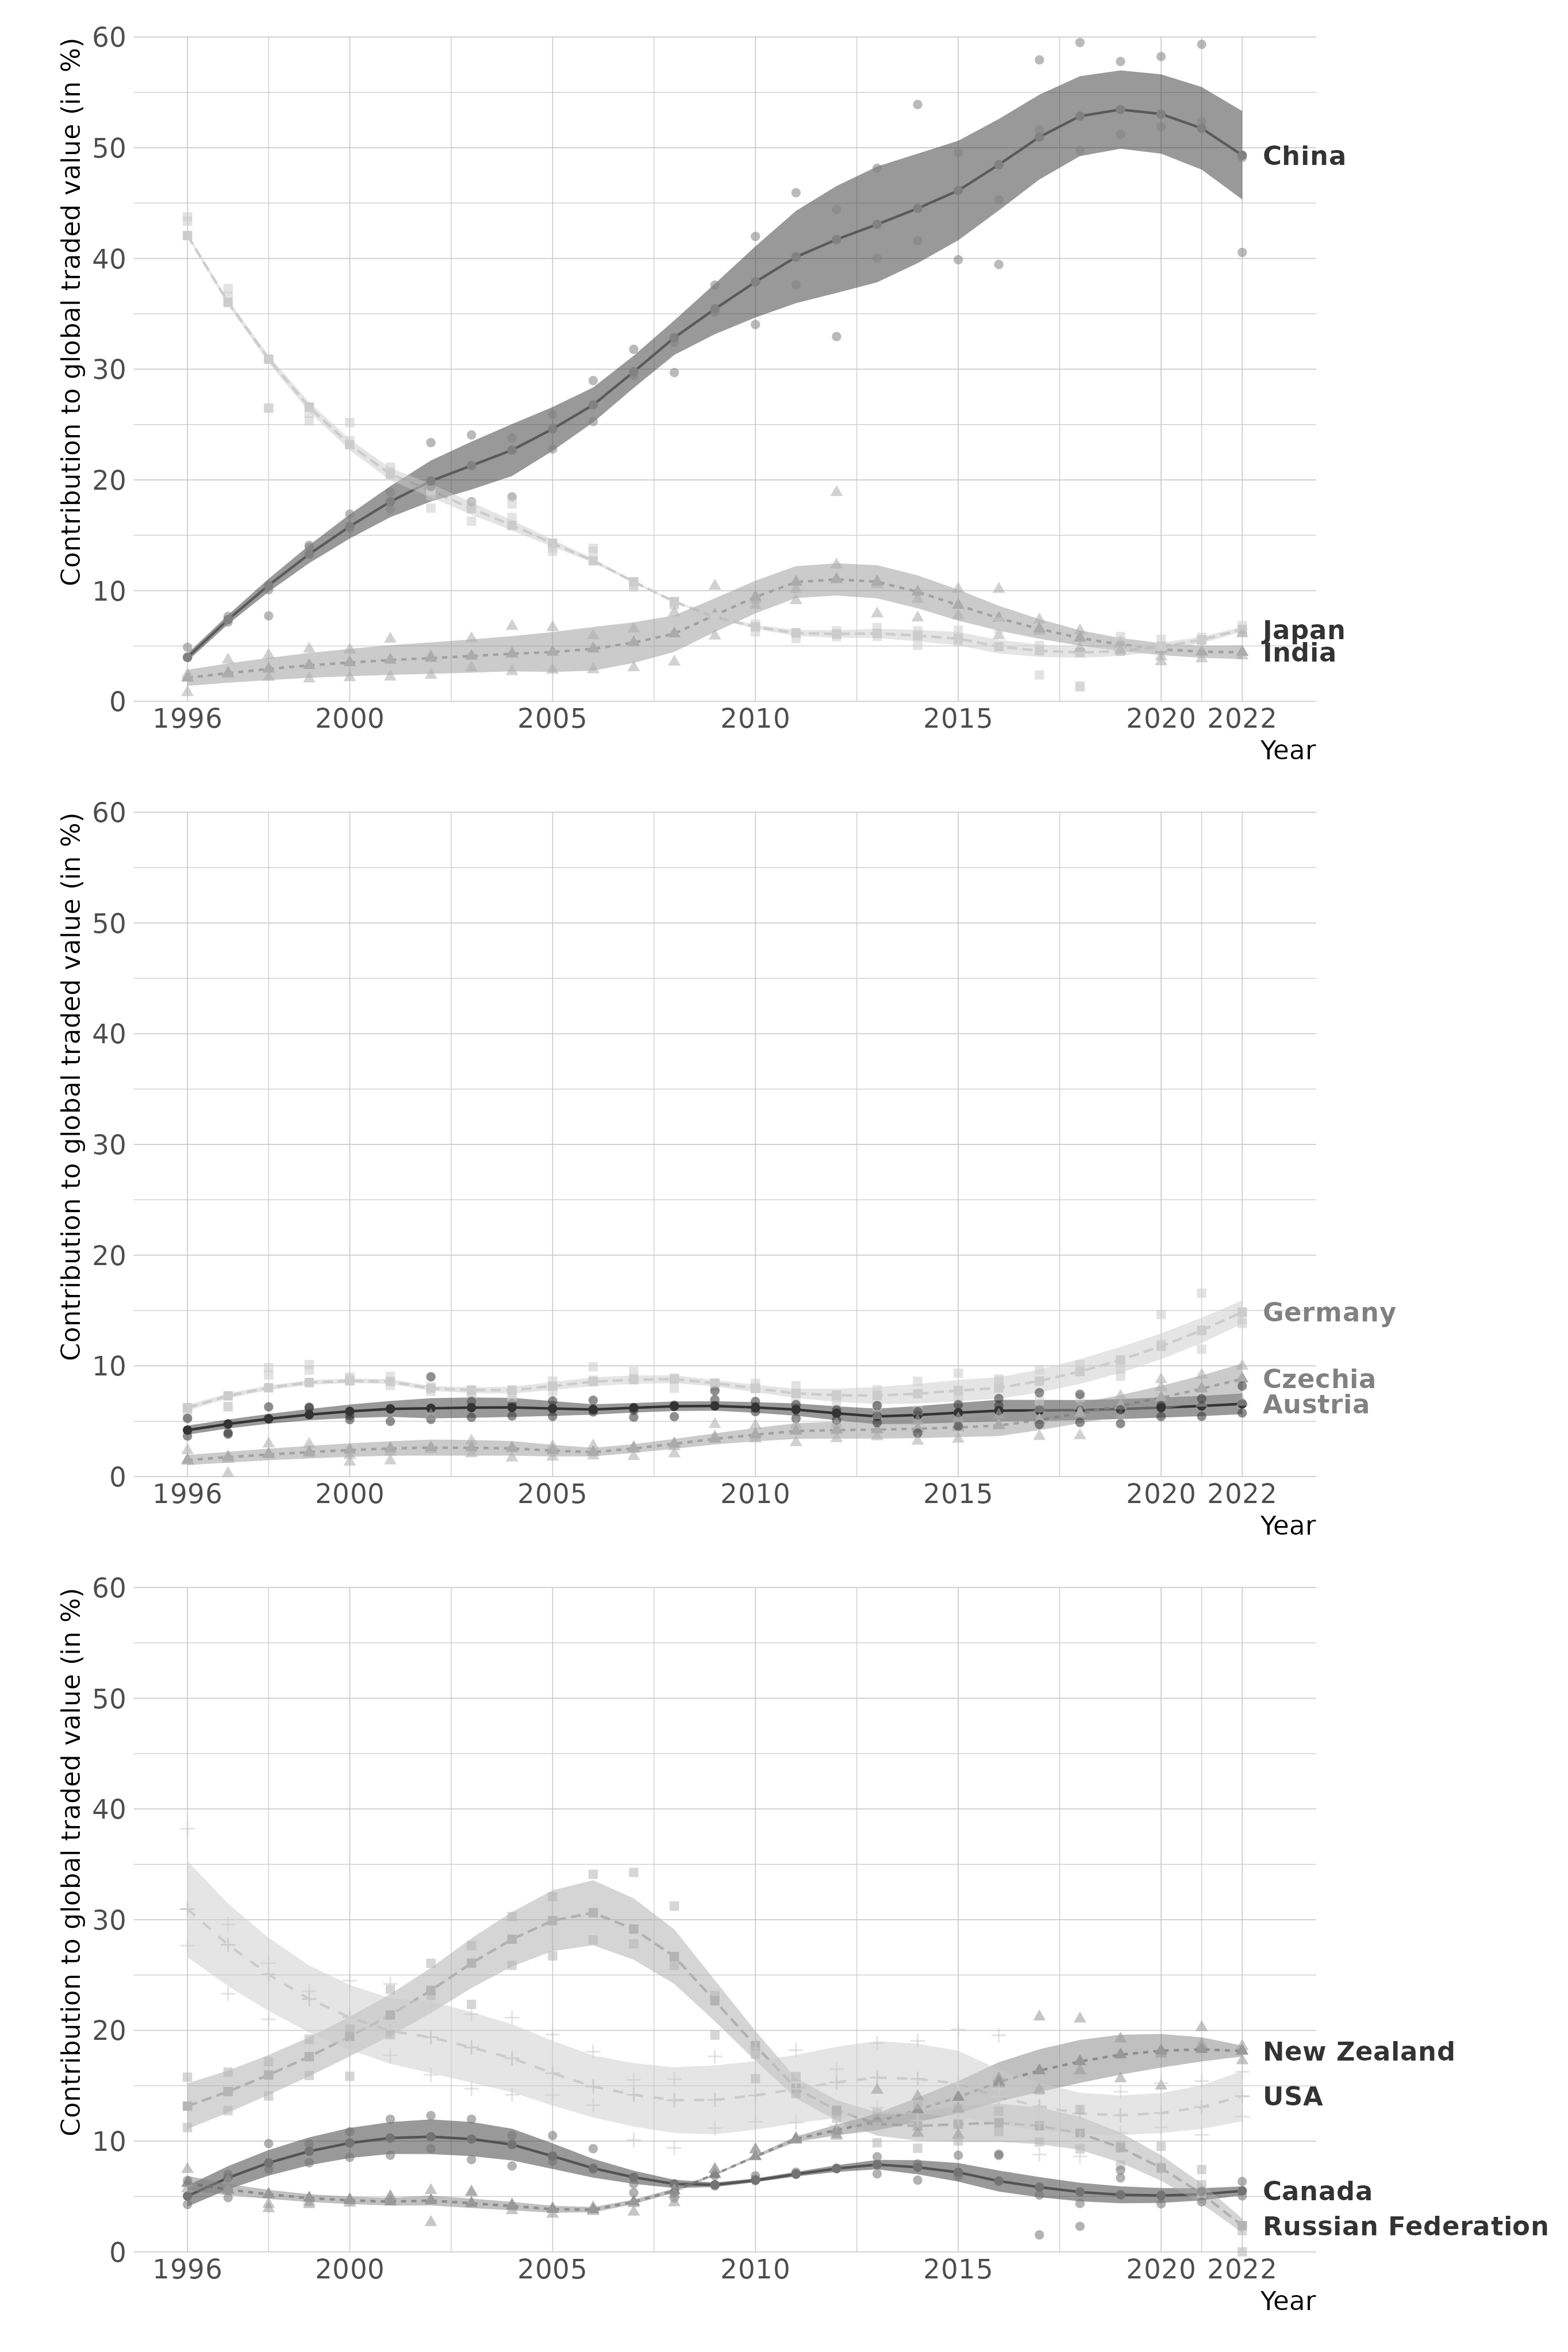
\includegraphics[width=\linewidth,height=0.9\textheight,keepaspectratio]{figures/fig-network-contribution.png}

}

\caption{\label{fig-network-contribution}Contribution of different
countries to the total traded value of the network. Only countries that
have contributed to more than 5\% of the total traded value at least
once during the study period are shown. The envelope corresponds to the
uncertainty in the reported values. Contributions are displayed by group
of countries: importers (top); mixed countries (middle); and exporters
(bottom).}

\end{figure}%

Contributions from individual countries to the total network trade value
provide a more detailed picture of market concentration
(Figure~\ref{fig-network-contribution}). These contributions correspond
to the proportion of the network's total trade value that would be lost
if a particular country is omitted from the network, \emph{i.e.}, the
proportion of total trade value flowing through that country. Over the
study period, only thirteen countries contributed at least 5\% to the
network's total trade value once. Referring to
Figure~\ref{fig-countries-profiles}, main contributors to the total
trade value can be divided into three groups: importers (China, India
and Japan); European countries (Germany, Czechia, Austria, Sweden,
France, Poland); and traditional wood exporters (Canada, New Zealand,
the Russian Federation, and the USA).

Among importers, Japan's share of total trade value decreased
considerably from around 44\% in 1996 to less than 6\% in 2023. On the
other hand, India's contribution increased steadily from around 2\% in
1996 to around 16\% in 2012, after decreasing to 6\% in 2023. Most
notably, China's share of the total trade value increased sharply, from
around 4\% in 1996 to more than 56\% in 2021, before decreasing to 44\%
in 2023. Together with results from Figures \ref{fig-countries-profiles}
and \ref{fig-market-concentration}, this indicated that around 56\% of
the total trade value flowed through China in 2021 due to its imports,
which is consistent with the high level of market concentration in
roundwood imports in over the past decade. The decline in the
concentration of roundwood imports since 2021 is likely due to China's
decreased trade contribution.

Germany stands out among European countries with a 14\% contribution to
trade in 2023. The Czech Republic, Austria, Sweden, France, and Poland
present similar contributions, between 5\% and 8\% in 2023. While
France's contribution to trade remained stable at around 4.7\% over the
study period, other European countries increased their contributions.
The contribution of Austria and Sweden moderatly increased from around
4\% in 1996 to 8\% and 7\% in 2023, respectively. The sharpest increases
in contributions to trade among European countries are observed for
Germany (rising from 6\% in 1996 to 14\% in 2023), the Czech Republic
(rising from 2\% in 1996 to 6\% in 2023), and Poland (rising from 0\% in
1996 to 5\% in 2023). These levels of contribution remain relatively low
compared to those of main importers such as China.

Among exporters, the contribution of the USA significantly decreased
over the studied period, falling from 33\% in 1996 to 13\% in 2007. It
then stabilized at an average of around 13.7\% over the 2007-2023
period. Canada's contribution to total trade value increased from 5\% in
1996 to 11\% in 2002, before decreasing to 6\% in 2007. It has remained
stable since then, averaging around 6.2\%. By contrast, New Zealand's
contribution initially slightly fell from 7\% in 1996 to 4\% in 1998,
then stabilised at an average of around 4.4\% between 1998 and 2008,
before rising significantly to 19\% in 2023. On the other hand, Russia
exhibits a unique pattern of varying contributions to the total trade
value throughout the studied period. Initially, Russian contributions
increased from 13\% in 1996 to 31\% in 2007, before dropping sharply to
12\% in 2012. This figure then stabilised at an average of around 11.4\%
between 2012 and 2018, before dropping again to below 1\% in 2023. This
correlates with findings presented in
Figure~\ref{fig-countries-profiles}, which suggests that Russian trade
integration has decreased over time. Except for Russia, which appears to
be influenced by short- to medium-term shocks, all contributors to the
roundwood trade exhibit long-term variations in their contribution.

\section{Conclusion and Discussion}\label{conclusion-and-discussion}

Contrary to our expectations, our results suggest that the global
roundwood trade network displayed significant resilience to exogenous
disruptions. Primarily, we show that the trade network followed its
long-term trend toward greater import concentration and polarization
around China, rather than experiencing major short-term shifts.
Interestingly, despite China's substantial growth in market power in
recent decades, our findings suggest that its influence on the roundwood
trade has declined in recent years, suggesting an impending shift.

Certainly, the network structural metrics showed low to moderate
sensitivity to shocks and disruptions. The number of pure exporters,
pure importers, and mixed countries, showed slight short-term drops over
the studied period (Figure~\ref{fig-network-composition}). Short-term
increases and decreases in connectivity or market concentration metrics
were also observed from year to year (Figures
\ref{fig-network-connectivity}, \ref{fig-market-concentration}). These
rises and falls in the network structure likely result from three broad
categories of events. First are economic disruptions, such as financial
or banking crises (\emph{e.g.}, the 2008 global financial crisis or the
2016 Chinese financial crisis) and supply chain disruptions
(\emph{e.g.}, the Covid-19 pandemic). Second are political events, such
as trade disputes
\citep{van_kooten_global_2014, johnston_impact_2017, pan_impacts_2021}
or bilateral agreements, which affect trade relationships between
countries. Third are ecological disasters. Hurricanes, tsunamis, and
earthquakes can result in direct and indirect damage, as well as periods
of reconstruction that can intensify the need for imports or the ability
to export. Forest fires and storms may affect the availability of
roundwood, thereby altering exports and imports throughout the supply
and production chains. However, these shocks seem to have no lasting
impact on the network structure, only affecting it in the short term,
with a quick recovery the following year. This suggests that the trade
network is resilient to exogenous shocks.

In fact, our results rather show that the roundwood trade network has
followed long-term trends over the past decades. In the long term, we
found that while the number of countries participating in the roundwood
trade network remained relatively stable, it underwent a notable shift
in composition, with countries engaging more in both exports and imports
(Figure~\ref{fig-network-composition}), suggesting a better integration
of countries in the network and trade intensification. Indeed, the
network's connectivity tightened at the turn of the 21st century
(Figure~\ref{fig-network-connectivity}), a trend consistent with broader
globalization \citep{prestemon_international_2003}. Our analysis of
network composition and connectivity further reveals an uneven
structure: a few highly-connected countries (the hubs) dominate and
concentrate trade, while most of the network consists of
poorly-connected countries that barely contribute to roundwood trade
volumes (Figures \ref{fig-countries-profiles},
\ref{fig-network-connectivity}). These hubs play a critical role in
network's functionality \citep{huang_static_2024} and can wield
considerable market power, with potential anti-competitive effects on
poorly-connected countries, which constitute the majority of the trade
network.

Throughout the study period, many major hubs in the international
market, including the USA, Canada, Western Europe, Scandinavia, and
Russia, maintained a high number of trading partners. However, our
findings highlight long-term shifts in the trade landscape over recent
decades. We observed a decline among traditional core importers and
exporters, including Japan, Russia, and the USA, concurrent with the
rise of new key players like China and New Zealand (Figures
\ref{fig-countries-profiles}, \ref{fig-network-contribution}).
Especially, our findings show that China has become \emph{the} central
player in the roundwood trade, substantially increasing its number of
import and export partners. By 2021, China's imports accounted for 56\%
of the total roundwood trade value, leading to a highly concentrated and
polarized import market (Figures \ref{fig-market-concentration},
\ref{fig-network-contribution}). This confirms findings from other
studies
\citep{ke_changes_2019, long_exploring_2019, zhou_spatial_2021, shen_structural_2022, huang_static_2024}.

This could appear as a paradox: although forest resources are
geographically concentrated in a few countries, our results show that
the roundwood export market is not similarly concentrated
(Figure~\ref{fig-market-concentration}). The relatively low export
market concentration levels observed during the last decade are
presumably due to Russia's withdrawal from the export market initiated
in 2007. The increase in export market concentration at the beginning of
the 20th century coincided with Russia's growing contribution to trade
(Figures \ref{fig-market-concentration},
\ref{fig-network-contribution}). In 2007, Russian roundwood exports
represented 34\% of the global roundwood export volumes. Russia
contribution to roundwood trade then fell from 31\% in 2007 to less than
1\% in 2023 due to successive export tax increases on roundwood, which
preceded a complete export ban in 2022
(Figure~\ref{fig-network-contribution})
\citep{lin_incidence_2017, unecefao_forest_2022, unecefao_forest_2022-1, fao_state_2024, guan_impact_2024}.
Russia's position as the main exporter of roundwood has since been
overtaken by New Zealand, which accounted for 20\% of total exports in
2023. In 2023, other roundwood exporters significantly contributed to
global export volumes: the USA (15\% of global roundwood exports),
Germany (10\%), Czechia (6\%), France and Canada (4\% each), Poland,
Latvia, and Norway (3\% each), and Papua New Guinea (2\%). Such
distribution of export volumes may explain the relatively low
concentration levels of the roundwood export market.

In contrast, our findings suggest that the import market has become
highly concentrated primarily due to demand from China (Figures
\ref{fig-market-concentration}, \ref{fig-network-contribution}), which,
paradoxically, also possesses the fifth-highest forest endowment and
presents the first-highest average annual net gain in forest area
\citep{fao_state_2024}. Indeed, due to Chinese government efforts in
spending, as well as China's market and policy reforms driven by forest
conservation demand, China has operated a drastic expansion of its
forestry and planted forest extensive margins over the last decades
\citep{demurger_forest_2009, ke_changes_2019, zhang_chinas_2019, zhao_large-scale_2022}.
However, despite an increase in China's forest area and volume, low
economic tree planting efficiency and poor forest management have
resulted in low stand quality and growth rates
\citep{hoffmann_adapting_2018, hou_intensifying_2019, ke_changes_2019, zhang_chinas_2019}.
As a result, domestic timber consumption --- primarily for industrial
and construction uses --- has outpaced domestic production, making China
highly dependent on imported wood products, which now account for
approximately half of its total timber supply
\citep{demurger_forest_2009, he_projection_2011, hoffmann_adapting_2018, hou_intensifying_2019, ke_changes_2019}.

Such demand for imported roundwood fosters co-dependence between China
and roundwood exporting countries. In fact, China serves as the main
trading partner for most major exporters, making them highly reliant on
its demand. For instance, in 2020, China imported 46\% of roundwood
exports from the USA, 67\% from Russia, 77\% from Congo, 78\% from Papua
New Guinea, and 86\% from New Zealand. The case of New Zealand perfectly
illustrates this co-dependence. Its rise as a major exporter is closely
tied to China's increasing demand and Russia's concurrent withdrawal
from the roundwood export market. The share of New Zealand's roundwood
exports to China surged from just 1.2\% in 1996 to 90.3\% in 2023. To
mitigate risks from potential disruptions caused by hubs like China or
to limit co-dependence, countries can diversify their trade
relationships \citep{huang_static_2024}. The United States appears to
have pursued this strategy throughout the study period, as shown in our
results (Figure~\ref{fig-countries-profiles}).

This overall suggests that roundwood trade flows are predominantly
demand-driven rather than supply-pushed. In the case of China, the
primary use of wood for industrial and construction uses
\citep{hou_intensifying_2019} echoes the role of population and
urbanization in shaping demand for materials
\citep{steinberger_global_2010}, which has been identified in the
literature
\citep{unecefao_forest_2022-1, mathieu_meta-analysis_2023, villamor_preparing_2024}.
Urbanization, through the growth, maintenance, and operation of
buildings, infrastructure, and durable goods, is a major determinant of
material consumption
\citep{fernandez_resource_2007, hu_input_2010, krausmann_global_2017, deetman_modelling_2020},
which may have a considerable impact on roundwood trade. Regions of the
world undergoing population increase and urbanization, such as emerging
markets in Asia \citep{deetman_modelling_2020, unecefao_forest_2022-1},
are or are becoming centers of gravity that attract roundwood trade
flows, with potential shifts in the role of countries within the trade
network.

Most interestingly, China's contribution to the roundwood trade appears
to have begun a decline after 2021
(Figure~\ref{fig-network-contribution}), potentially signaling a new
phase in the global roundwood market. Three concurrent and reinforcing
circomstances may drive this decline: external geopolitical disruptions,
domestic self-sufficiency policies, and domestic structural economic
changes.

The initial decline likely stems from major external trade shocks. Most
notably, Russia's 2022 roundwood export ban significantly reduced
China's import volumes; in 2021, Russia was China's third main supplier,
accounting for 7.2\% of its roundwood imports (a share that fell to
3.2\% in 2022). Consequently, China appears to be shifting its import
strategy from raw logs to processed wood products, absorbing significant
volumes of Russian plywood, for example, that were previously destined
for Western markets following Ukraine war-related sanctions
\citep{scott_against_2024}. This shock was likely exacerbated by the
still ongoing 2018 US-China trade war
\citep{muhammad_end_2021, pan_impacts_2021}. While the U.S. share of
China's imports increased from 8.5\% in 2021 to 10.9\% in 2023 (possibly
to compensate for Russian withdrawal from the export market), China's
import volume from the U.S. has dropped by 29\% over the same period.
Given the current geopolitical climate, a Russian ban lift is unlikely,
and escalating U.S.-China trade barriers are expected to cause further
significant trade disruptions and diversions in the medium term
\citep{attinasi_navigating_2024, world_bank_global_2025, world_trade_organization_global_2025}.

A second, more policy-driven factor is China's strategic ambition to
enhance self-sufficiency and reduce reliance on wood imports by relying
on domestic demand and more comprehensive domestic supply chains
\citep{fao_society_2021, unecefao_forest_2022-1, attinasi_navigating_2024}.
High reliance on imports, particularly with sourcing concentration risks
intensifying, presents geopolitical risks for China. In this regard,
China announced its Plan for the Construction of the National Reserve
Forest Project in 2018. This project aims to foster a net increase of
200 million m\textsuperscript{3} per year by 2035 from 20 million newly
planted hectares of national reserve forest-an amount designed to cover
China's current total net imports of forest products. This domestic
focus aims to make the country less export-oriented and mitigate
sourcing risks.

Thirdly, China's contribution decline in roundwood trade network may
result from demestic economic crisis and structural changes. For the
last four years, China has known a real estate crisis which, coupled
with slowed productivity growth, ageing population and high debt levels,
has significantly slowed its domestic demand for roundwood
\citep{world_bank_global_2025}, which again echoes the role of
urbanization in fueling demand for materials such as wood. Furthermore,
while China's position in global value chains has been fueled by
labour-intensive industry development \citep{su_assessment_2020},
last-decades increases in labour costs and investments in research and
development towards advanced technologies has led China to pivot from
consumer goods production and exports to technology-intensive capital
production and exports
\citep{fao_society_2021, attinasi_navigating_2024}. In fact,
labour-intensive consumer goods production is currently moving out of
China, such as Vietnam
\citep{fao_society_2021, attinasi_navigating_2024}.

Finally, the decline may be compounded by domestic economic crises and
structural shifts. Over the past four years, the real estate crisis in
China, coupled with slower productivity growth, an aging population, and
high debt levels, has significantly dampened domestic demand for
roundwood \citep{world_bank_global_2025}, which again highlights the
role of urbanization in driving demand for materials such as wood.
Furthermore, China is undergoing a structural pivot: driven by rising
labor costs and investments in research and development towards advanced
technologies, China is shifting from labor-intensive consumer goods
production and exports \citep{su_assessment_2020} to
technology-intensive capital production and exports
\citep{fao_society_2021, attinasi_navigating_2024}.\footnote{In fact,
  labour-intensive consumer goods production is currently moving out of
  China, to countries such as Vietnam
  \citep{fao_society_2021, attinasi_navigating_2024}.} This structural
change inherently reduces the domestic manufacturing sector's demand for
imported roundwood.

In light of these persistent factors, China's declining integration into
the roundwood trade network is likely to continue. A potential
``post-China'' era in the global roundwood market raises crucial
concerns: the potential contours of a fragmented trade world marked by
policy uncertainty
\citep{attinasi_navigating_2024, world_trade_organization_global_2025}
and the necessity of identifying new, sustainable markets for timber
supply for major exporters, such as New Zealand
\citep{villamor_preparing_2024}.

By considering multiple network metrics, we obtained a clearer picture
of the evolution of the network's structure than using a single metric
alone \citep{shanafelt_-it-yourself_2017, salau_taking_2022}. The mean
number of connections gives us a global measure of network connectivity,
but tells nothing of the distribution of connections throughout the
network. By measuring variance, skewness, and kurtosis we observed
changes in the variation of connections per node, the proportion of
poorly to highly-connected nodes, and the scarcity or abundance of
countries that diverge from the mean connectivity over time. This
provides a thorough diagnosis of the situation of the trade network. As
a complement to traditional market concentration indexes, measuring a
country's contribution to traded value provides a detailed overview of
each trader's relative market power. It is crucial to recognize that
network analysis should not be viewed as a replacement for traditional
methods but rather as a powerful complement. It offers a macro-level,
systemic perspective that can inform and enrich the micro-level insights
derived from econometric models or the aggregate flow analyses from
gravity models. Such multi-methodological approach would allow to
leverage the strengths of each technique, leading to a more holistic and
robust understanding of complex trade phenomena.

However, our results show that, despite the powerful explanatory
capacity of network analysis, the quality of the underlying trade data
is paramount. The validity and interpretability of the results are
directly influenced by the accuracy, completeness, and consistency of
the data, as pointed out in the literature
\citep{lovric_social_2018, wang_exploratory_2020, zhou_spatial_2021, huang_static_2024}.
While network analysis partly deals with data discrepancies by
simultaneously taking into account exports and imports, it reveals data
discrepancies such as inconsistent reporting, missing values, and
outliers \citep{kallio_reliability_2018, chen_advancing_2022}. Hence,
our results show that China exported roundwood to 32 more countries in
2020 compared to 2000, while simultaneously reporting a decrease of
\$1.2 million in export value on the same period (a decline of about
16\%), which seems unlikely (Figure~\ref{fig-countries-profiles}). This
further highlights the caution that should be brought by modelers and
data scientists when analysing bilateral trade data, while emphasizes
the need for methods to process trade data and correct quality issues or
for harmonized and consistent databases
\citep{gaulier_baci_2010, rougieux_forest_2017}.

Similarly, our results suggest that the country-level perspective is not
always the most relevant in trade analysis. In particular, results
highlight the singular trade balance of many European countries, which
export as much roundwood as they import. This would suggest to rather
consider the European Union as a whole, in order to get a clear vision
that is not blurred by individual European countries behaviours and that
will better reflect the European continent's trade weight and openess.

While network analysis captures complexity and describes its
organisation, further exploration of the determinants and dynamics is
necessary to understand the rules that govern trade organisation, as
well as to develop a unified indicator system, as network metrics are
diverse. Multi-layer networks, in particular, could provide a more
comprehensive analysis of global wood product supply chains by linking
each wood product network according to value chain logics.

\section*{References}\label{references}
\addcontentsline{toc}{section}{References}

\renewcommand{\bibsection}{}
\bibliography{references.bib}

\newpage{}

\section{Information}\label{information}

\subsection{Funding statement}\label{funding-statement}

This study was supported by two grants from the French Grand Est Region
(N° 19\_GE8\_019 20P05044) and the Lab of Excellence ARBRE (N°
WP4/20PN17), by the French National Research Institute for Agriculture,
Food and Environment (INRAE), and by AgroParisTech.

\subsection{CRediT authorship contribution
statement}\label{credit-authorship-contribution-statement}

Valentin Mathieu: Conceptualization, Methodology, Software, Validation,
Formal analysis, Investigation, Data Curation, Writing - Original Draft,
Writing - Review \& Editing, Visualization, Supervision, Project
administration.

David W. Shanafelt: Conceptualization, Methodology, Formal analysis,
Investigation, Writing - Original Draft, Writing - Review \& Editing,
Supervision.

\subsection{Declaration of competing
interest}\label{declaration-of-competing-interest}

The authors declare that they have no known competing financial
interests or personal relationships that could have appeared to
influence the work reported in this paper.

\subsection{Declaration of generative AI and AI-assisted technologies in
the writing
process}\label{declaration-of-generative-ai-and-ai-assisted-technologies-in-the-writing-process}

During the preparation of this work the authors used (1) Asta in order
to review the litterature aside traditional litterature search tools
such as Scopus and Google Scholar and (2) Gemini and DeepL tools to
improve English writing. After using this tool/service, the authors
reviewed and edited the content as needed and take full responsibility
for the content of the publication.

\subsection{Data availability}\label{data-availability}

Data and code are available on
\href{https://github.com/vlmathieu/trade_network_analysis}{GitHub}.

\subsection{Acknowledgements}\label{acknowledgements}

We thank Felix Bastit and Clément Nedoncelle for their helpful and
relevant comments and suggestions, as well as the following audience:
BETA internal environment, Labex ARBRE, Chaire RENEL, the 9th annual
conference of the French Association of Environmental and Resource
Economists (FAERE), DEEPSURF 2022 Energy and Ecological transition
international conference, and the 16th social science research days
(JRSS), Paris-Saclay Conference on Trade and Environment, 26th World
Congress of the International Union of Forest Research Organizations
(IUFRO) - Forests and Society towards 2050. All remaining errors are our
own.





\end{document}
